\chapter{Results and Observations}
\lhead{\emph{Results and Observations}}

In this section, the results of the experiments that have been conducted are presented. For each experiment, we will outline how the experiment was set up, what technologies we are testing and also give an unbiased overview of the data gathered.

\section{Stress Testing Multiple Language Implementations}

In this experiment, various implementations of web socket servers will be tested using the platform that has been created. Two web socket applications have been created for this. The first one is built using NodeJS, the second is built using GoLang. The purpose of this test is to demonstrate that the ws-flare platform can test web sockets written in multiple languages.

Before conducting each experiment, the ws-flare-platform has been deployed to a GKE Kubernetes cluster. The resources assigned to this cluster are defined in table \ref{table:kubernetes-setup-experminent-1}. The cost of running such a server for 24 hours a day are approximately 137 euro a month.

\begin{table}[H]
\resizebox{\textwidth}{!}{%
\begin{tabular}{llll}
\rowcolor[HTML]{ECF4FF} 
Machine Type          & Nodes & Total VCpus & Total Memory \\
small (1 Shared VCpu) & 10    & 10          & 16.99GB     
\end{tabular}%
}
\caption{Kubernetes Setup}
\label{table:kubernetes-setup-experminent-1}
\end{table}

\subsection{NodeJS Websocket Server}

For NodeJS we will be using a popular library called WS. The code for the server is outlined in listing \ref{table:nodejs-server-experiment-1}

\begin{listing}[H]
    \caption{NodeJS Websocket Server Implemntation}
    \label{table:nodejs-server-experiment-1}
    \begin{minted}{Javascript}
const http = require('http');
const WebSocket = require('ws');

console.log('Starting ws server');

const server = http.createServer();
const wss = new WebSocket.Server({noServer: true});

wss.on('connection', (ws) => {
    console.log('new connection');

    ws.on('close', () => {
        console.log('connection dropped');
    });
});

server.on('upgrade', function upgrade(request, socket, head) {
    wss.handleUpgrade(request, socket, head, function done(ws) {
        wss.emit('connection', ws, request);
    });
});

server.listen(process.env.PORT || 3000);
\end{minted}
\end{listing}

The NodeJS server as outline in listing \ref{table:nodejs-server-experiment-1}. One important node is that the code required to handle HTTP upgrades to web socket manually as Cloud Foundry does not automatically handle the HTTP upgrade. Without this hook it is not possible run a web socket server on Cloud Foundry. 

The NodeJS web socket server is deployed on cloud foundry with the resource limits specified in table \ref{table:cf-resource-limits-1}

\begin{table}[H]
\resizebox{0.7\textwidth}{!}{%
\begin{tabular}{ll}
\rowcolor[HTML]{ECF4FF} 
Instances & Memory Limit Per Instance \\
1         & 64MB                     
\end{tabular}%
}
\caption{Cloud Foundry Resource Limits}
\label{table:cf-resource-limits-1}
\end{table}

A diagram of the test to be conducted is shown in figure \ref{fig:experiment-1-vis-nodejs}

\begin{figure}[H]
  \centering
  \caption{Experiment setup for NodeJS server}
    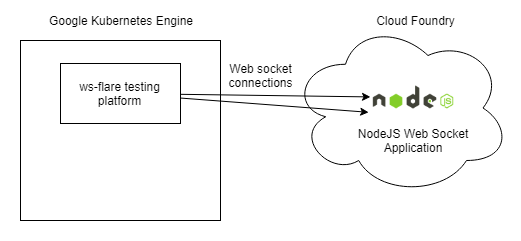
\includegraphics[width=0.8\textwidth]{figures/experiments/experiment-vis-nodejs.png}
    \label{fig:experiment-1-vis-nodejs}
\end{figure}

\subsubsection{Simulating 1000 connections}
The initial test uses the ws-flare script defined in listing \ref{table:nodejs-server-experiment-1} to simulate 1000 users over a period of 60 seconds

\begin{listing}[H]
    \caption{WS-Flare test script for 1000 users}
    \label{table:nodejs-server-experiment-1}
    \begin{minted}{json}
[
    {
        "start": 0,
        "timeout": 60,
        "totalSimulators": 1000,
        "target": "wss://ws-flare-test-server.cfapps.io:4443"
    }
]
\end{minted}
\end{listing}

\begin{figure}[H]
  \centering
    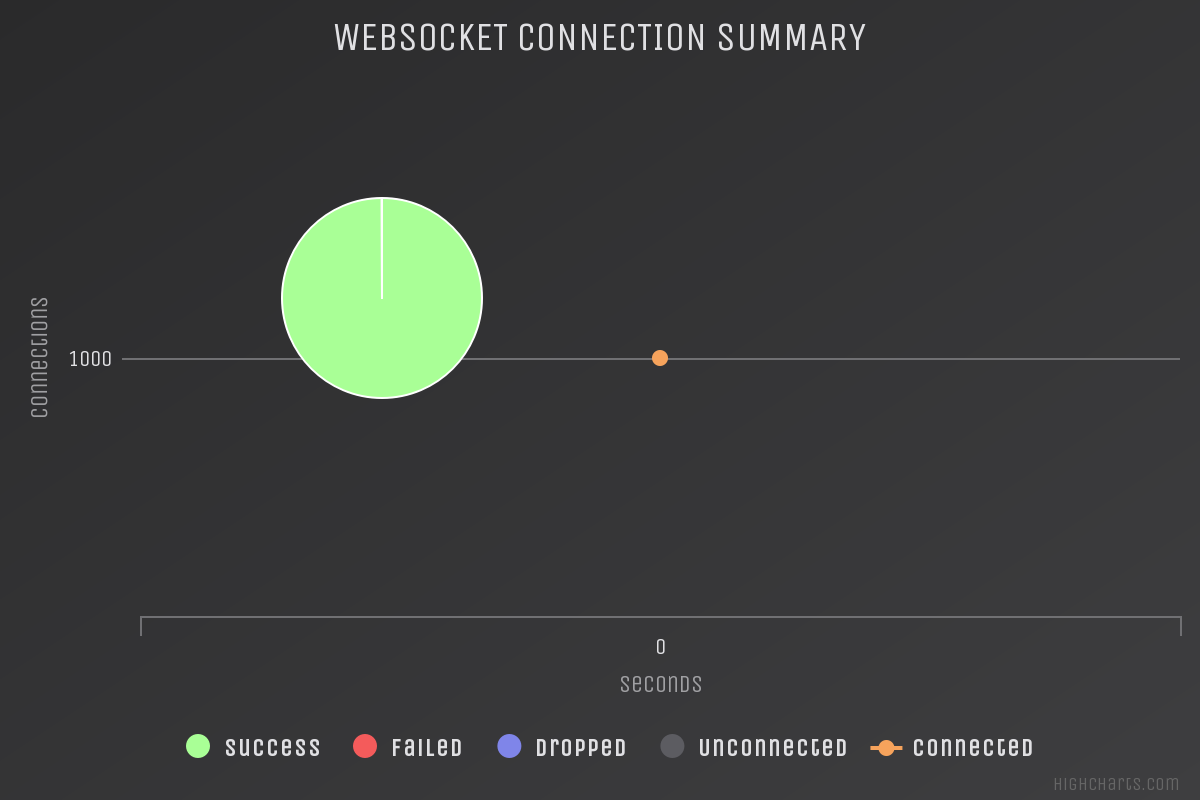
\includegraphics[width=0.8\textwidth]{figures/experiments/experiment-1/node-js/conn-summary-1000.png}
    \caption{Results of simulating 1000 websockets}
    \label{fig:experiment-1-node-conn-summary-1000}
\end{figure}

\begin{figure}[H]
  \centering
    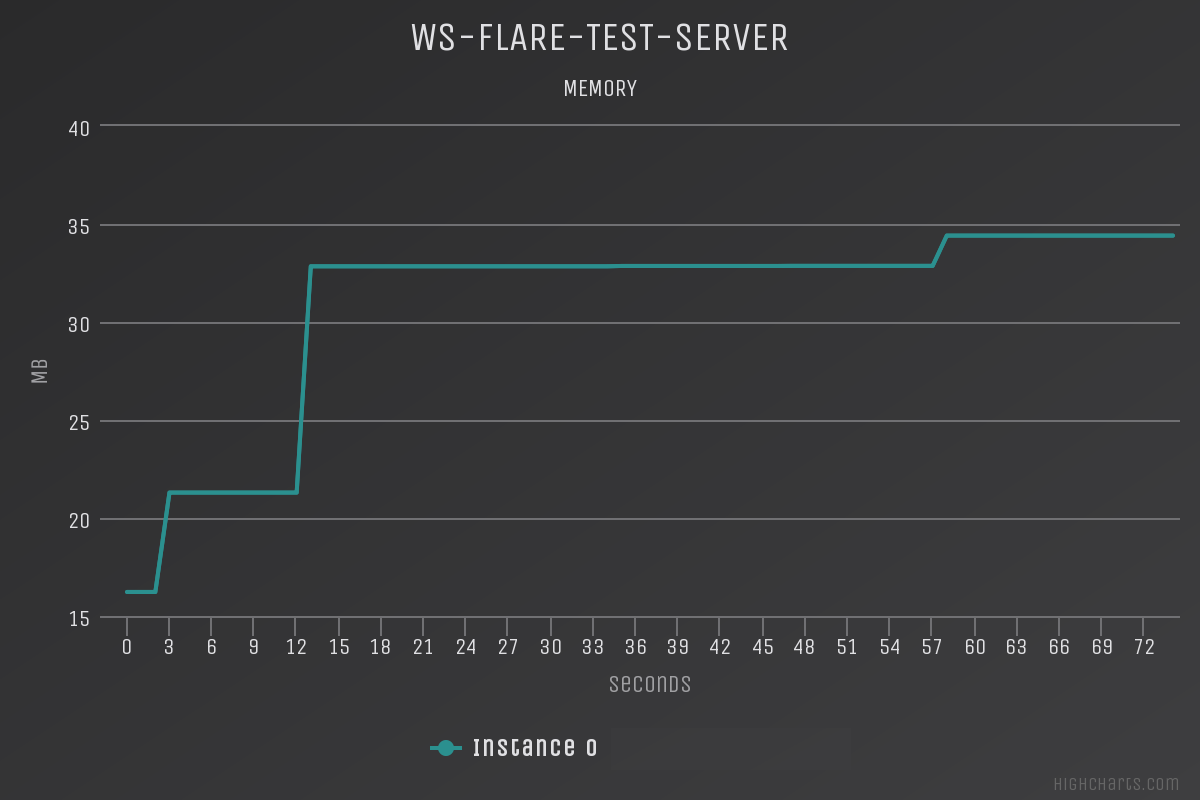
\includegraphics[width=0.8\textwidth]{figures/experiments/experiment-1/node-js/memory-1000.png}
    \caption{Memory consumption of websocket server testing 1000 connections}
    \label{fig:experiment-1-node-memory-1000}
\end{figure}

\begin{figure}[H]
  \centering
    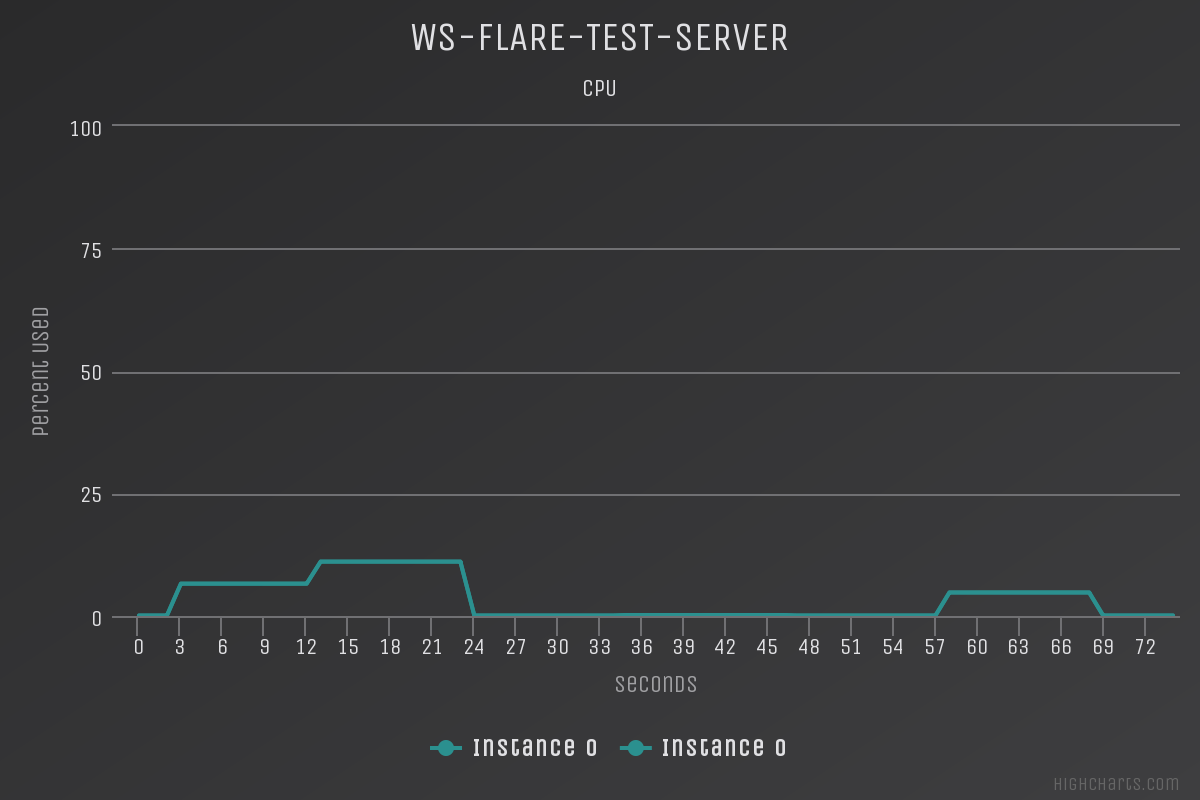
\includegraphics[width=0.8\textwidth]{figures/experiments/experiment-1/node-js/cpu-1000.png}
    \caption{CPU consumption of websocket server testing 1000 connections}
    \label{fig:experiment-1-node-cpu-1000}
\end{figure}

As can be seen from figure \ref{fig:experiment-1-node-conn-summary-1000} simulating 1000 users has a 100\% success rate.

In figure \ref{fig:experiment-1-node-memory-1000} and figure \ref{fig:experiment-1-node-cpu-1000} the memory and CPU resources are outlined as the test is in progress. We can see that the memory gradually rises from 16(MB) to 34 (MB). The CPU consumption remains stable throughout the test, reaching a maximum of 11\% usage. This occurred as the web sockets were initializing the connection to the server, suggesting that the most resource intensive time occurs when making the initial connection. After all connections have been made we then see the CPU return to 0\% usage. 

\subsubsection{Simulating 5000 Connections}

1000 users connecting at the same time is a good expectation for websites that are not expecting a lot of traffic. To increase the total connections to 5000, the script in listing \ref{table:nodejs-server-experiment-2} is used.

\begin{listing}[H]
    \caption{WS-Flare test script for 5000 users}
    \label{table:nodejs-server-experiment-2}
    \begin{minted}{json}
[
    {
        "start": 0,
        "timeout": 60,
        "totalSimulators": 5000,
        "target": "wss://ws-flare-test-server.cfapps.io:4443"
    }
]
\end{minted}
\end{listing}

\begin{figure}[H]
  \centering
    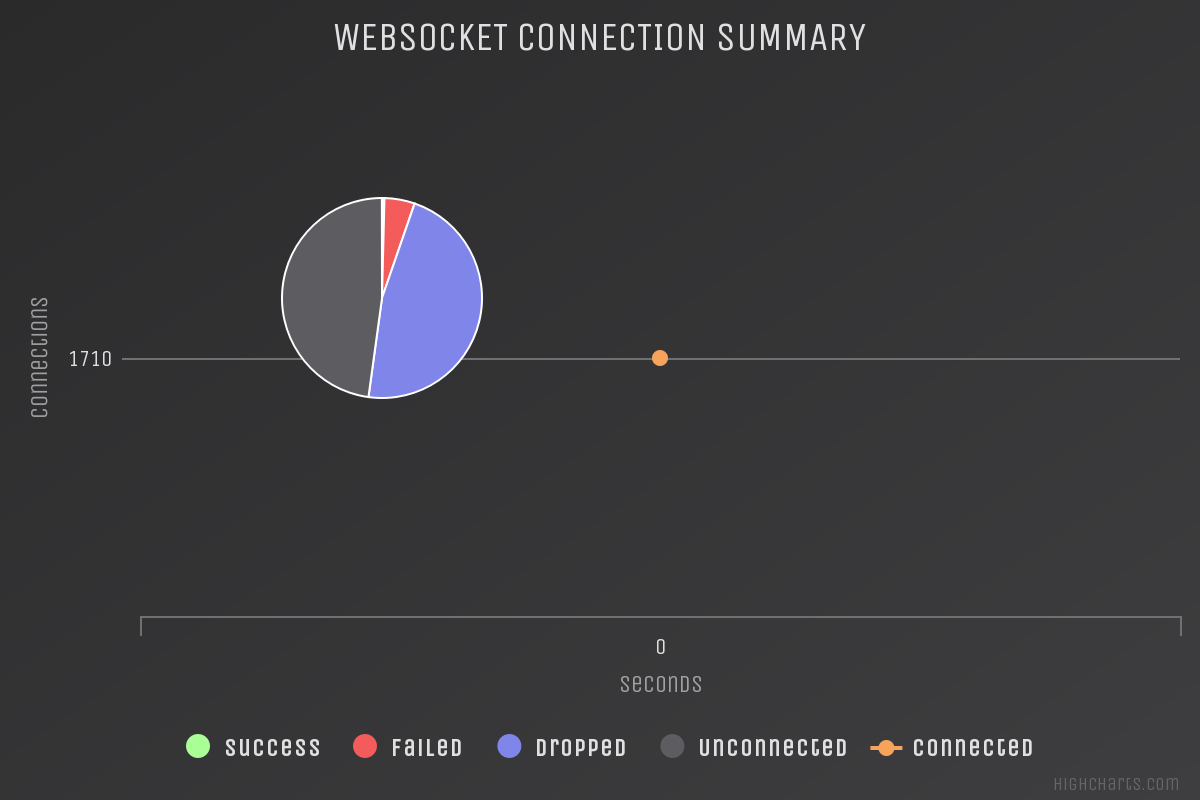
\includegraphics[width=0.8\textwidth]{figures/experiments/experiment-1/node-js/conn-summary-5000.png}
    \caption{Results of simulating 5000 websockets}
    \label{fig:experiment-1-conn-summary-5000}
\end{figure}

\begin{figure}[H]
  \centering
    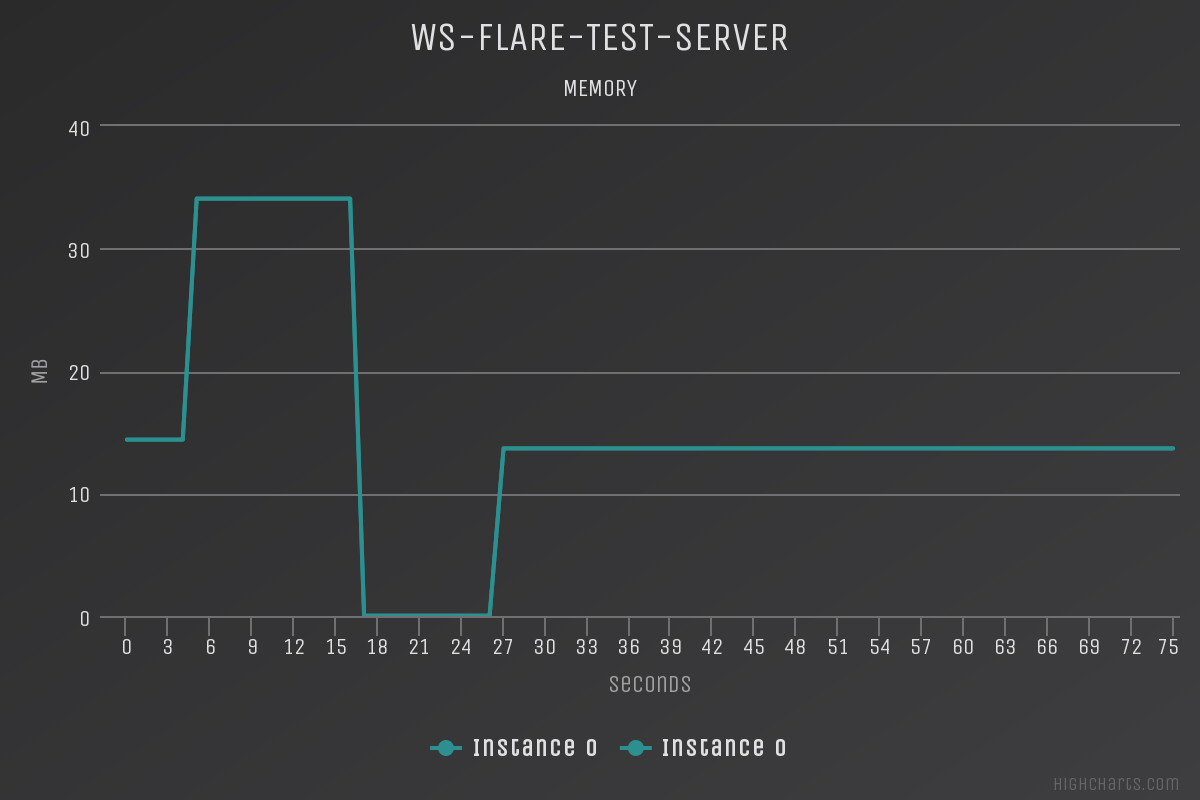
\includegraphics[width=0.8\textwidth]{figures/experiments/experiment-1/node-js/memory-5000.png}
    \caption{Memory consumption of websocket server testing 5000 connections}
    \label{fig:experiment-1-memory-5000}
\end{figure}

\begin{figure}[H]
  \centering
    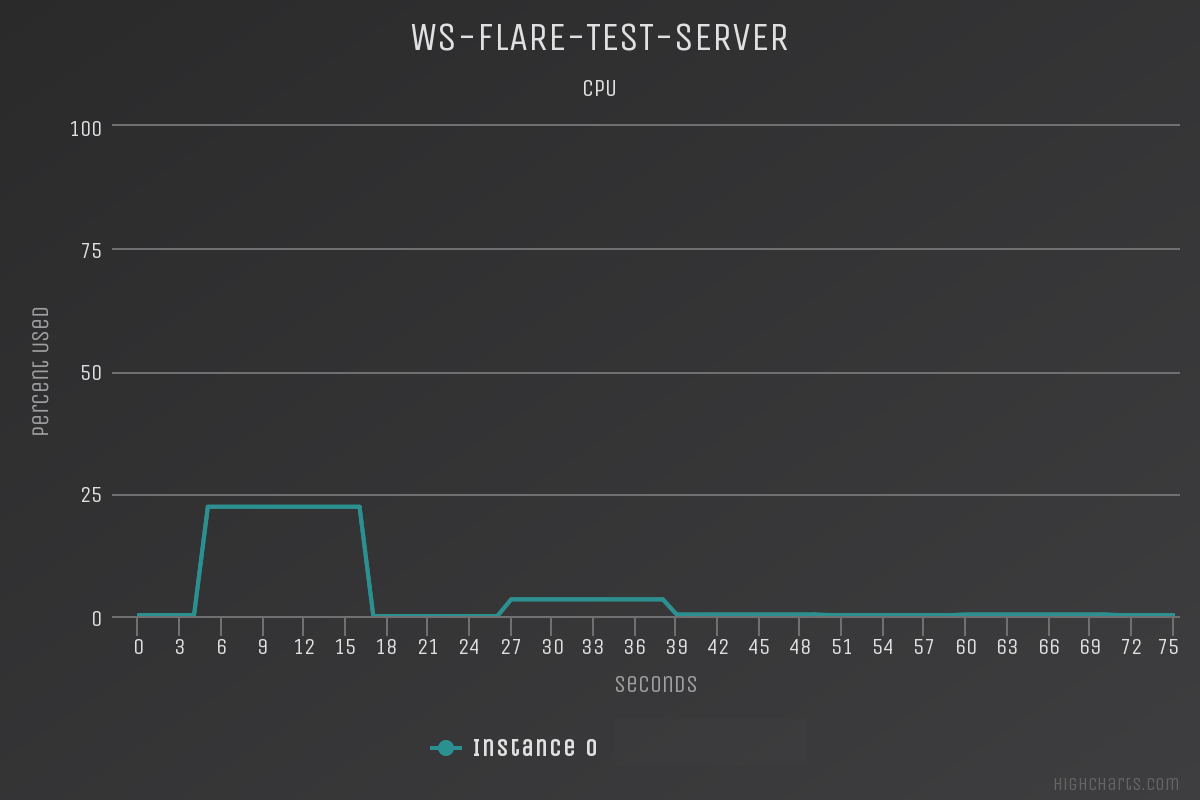
\includegraphics[width=0.8\textwidth]{figures/experiments/experiment-1/node-js/cpu-5000.png}
    \caption{CPU consumption of websocket server testing 5000 connections}
    \label{fig:experiment-1-cpu-5000}
\end{figure}

After increasing the test to simulate 5000 connections it can be seen in figure \ref{fig:experiment-1-conn-summary-5000} that initially the test reached 1710 connections. After this was reached there a large drop in memory as seen in figure \ref{fig:experiment-1-memory-5000} and CPU in figure \ref{fig:experiment-1-cpu-5000}. The indicates that a 64(MB) limit of memory is not enough to handle 5000 web socket connections. One possible solution to this is to add more instances. Through experimentation, it was found that to reach 5000 users successfully connecting at the same time, one of the resources defined in table \ref{table:cf-resource-limits-3} are needed on Cloud Foundry.

\begin{table}[H]
\resizebox{0.7\textwidth}{!}{%
\begin{tabular}{ll}
\rowcolor[HTML]{ECF4FF} 
Instances & Memory Limit Per Instance \\
4         & 64MB     \\
1         & 256MB     
\end{tabular}%
}
\caption{Cloud Foundry Resource Limits}
\label{table:cf-resource-limits-3}
\end{table}

\begin{figure}[H]
  \centering
    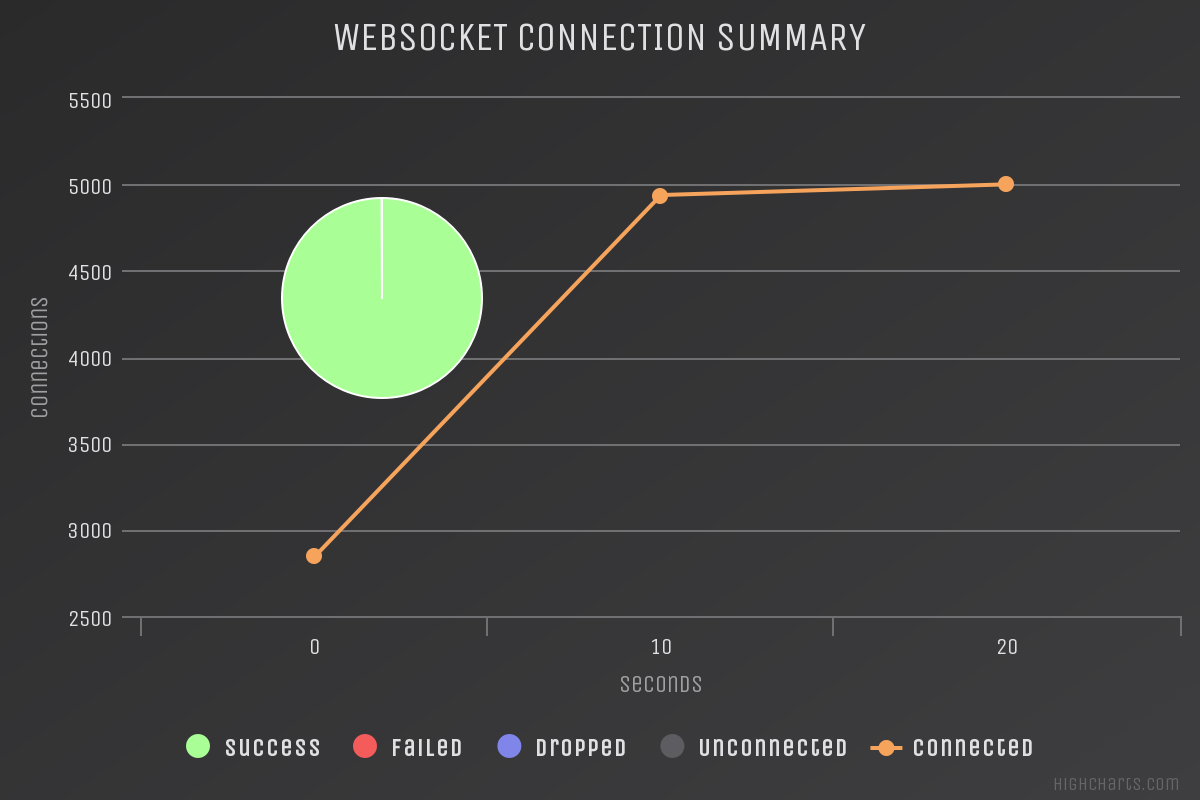
\includegraphics[width=0.8\textwidth]{figures/experiments/experiment-1/node-js/conn-summary-5000-4-instances.png}
    \caption{Results of simulating 5000 websockets with 4 instances}
    \label{fig:experiment-1-conn-summary-5000-4-instances}
\end{figure}

\begin{figure}[H]
  \centering
    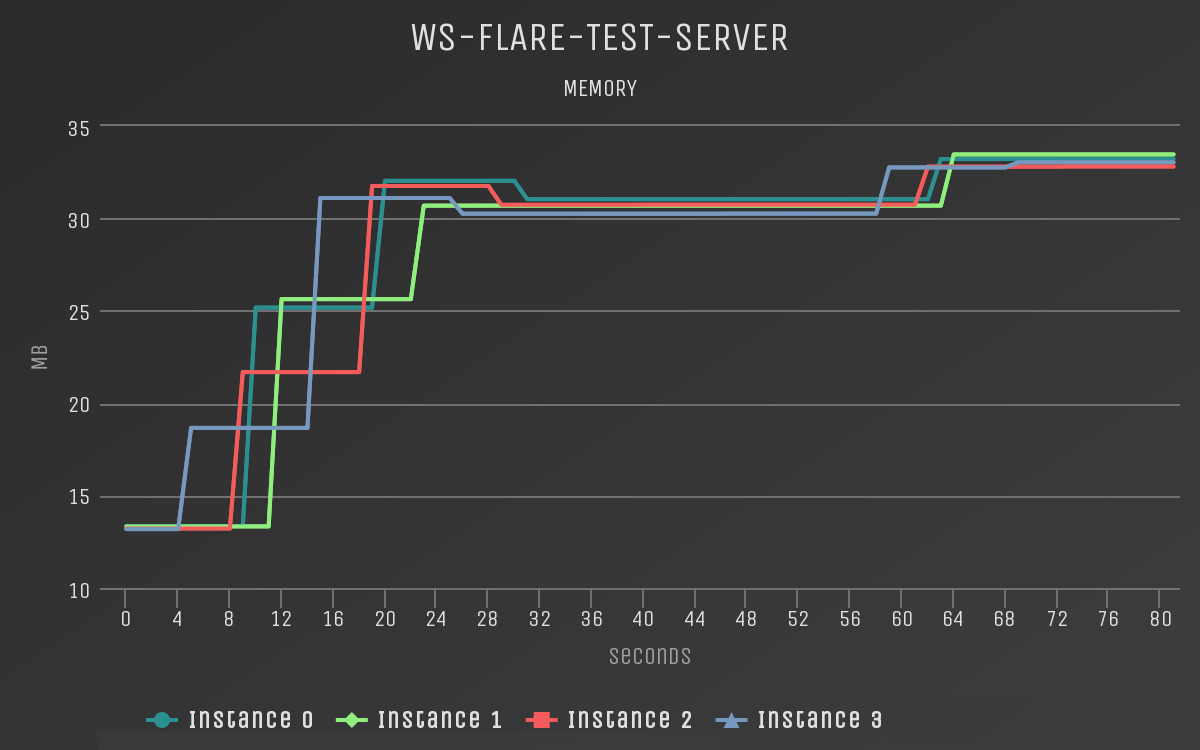
\includegraphics[width=0.8\textwidth]{figures/experiments/experiment-1/node-js/memory-5000-4-instances.png}
    \caption{Memory consumption of websocket server testing 5000 connections with 4 instances}
    \label{fig:experiment-1-memory-5000-4-instances}
\end{figure}

\begin{figure}[H]
  \centering
    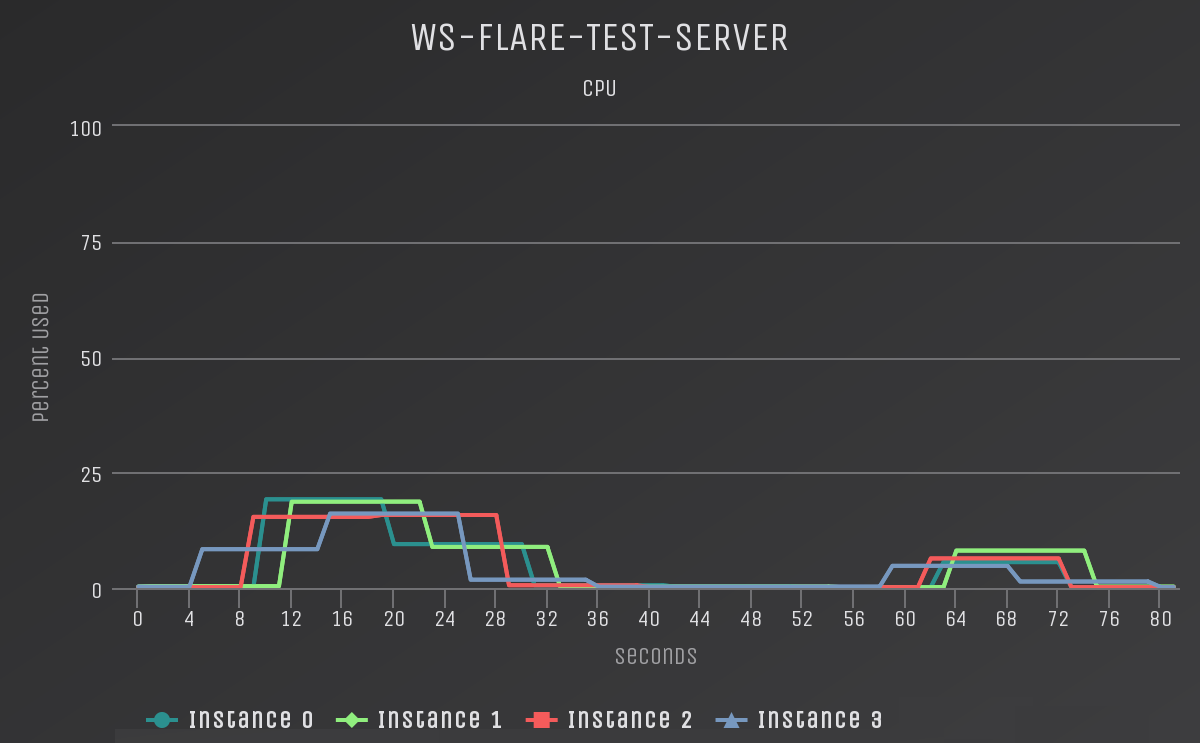
\includegraphics[width=0.8\textwidth]{figures/experiments/experiment-1/node-js/cpu-5000-4-instances.png}
    \caption{CPU consumption of websocket server testing 5000 connections with 4 instances}
    \label{fig:experiment-1-cpu-5000-4-instances}
\end{figure}

\begin{figure}[H]
  \centering
    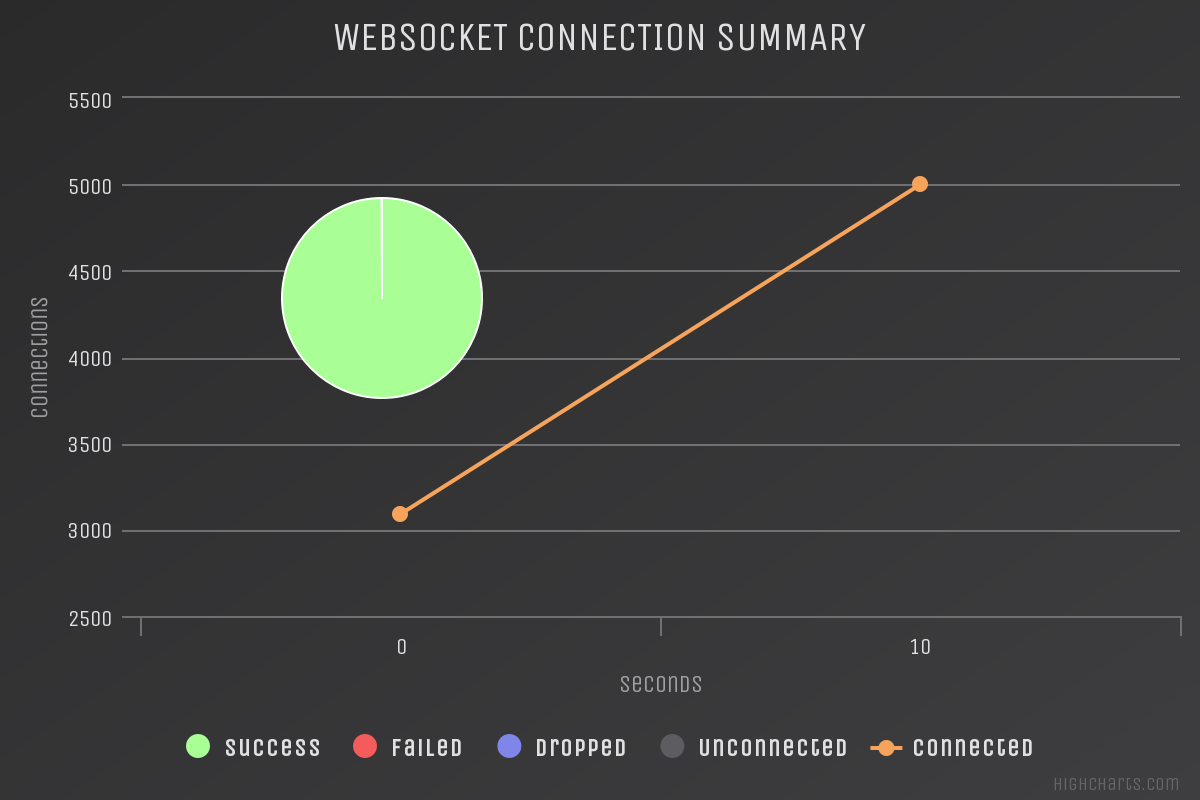
\includegraphics[width=0.8\textwidth]{figures/experiments/experiment-1/node-js/conn-summary-5000-256-memory.png}
    \caption{Results of simulating 5000 websockets with 256 MB of memory}
    \label{fig:experiment-1-conn-summary-5000-1-instances-256-mem}
\end{figure}

\begin{figure}[H]
  \centering
    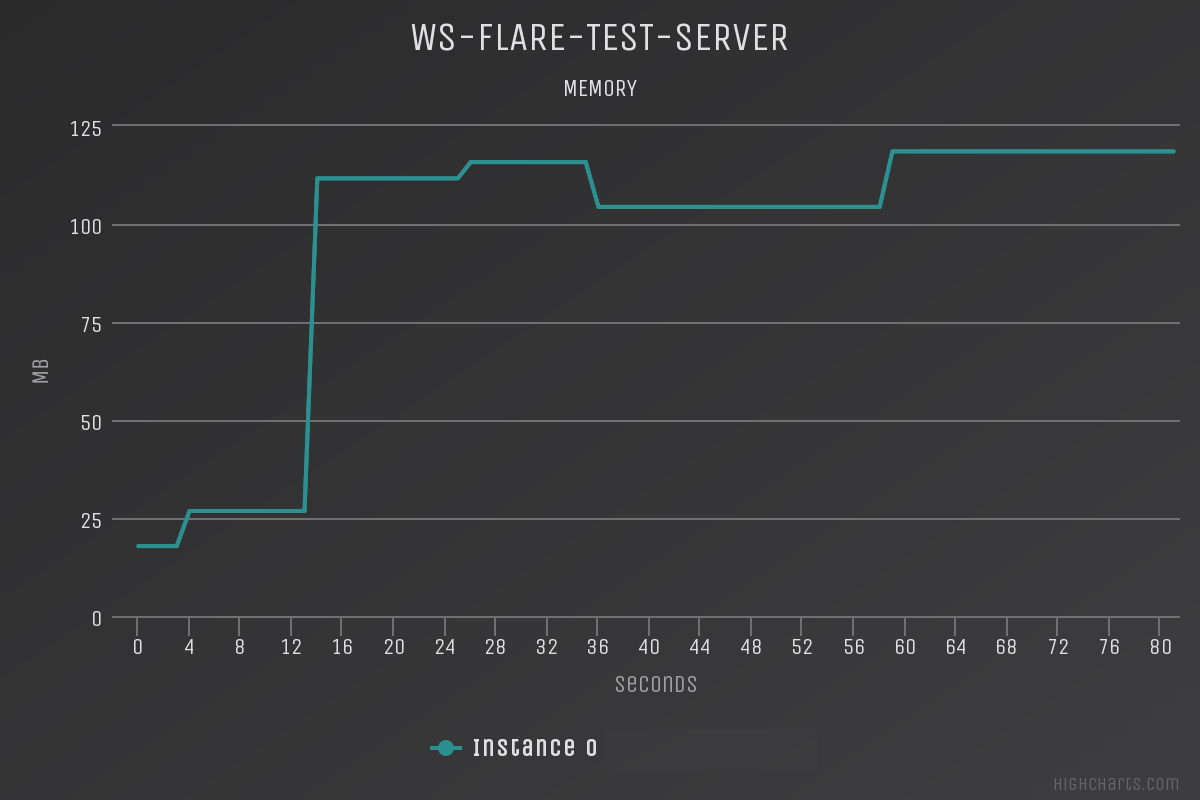
\includegraphics[width=0.8\textwidth]{figures/experiments/experiment-1/node-js/memory-5000-256-memory.png}
    \caption{Memory consumption of websocket server testing 5000 connections with 256 MB of memory}
    \label{fig:experiment-1-memory-5000-1-instances-256-mem}
\end{figure}

\begin{figure}[H]
  \centering
    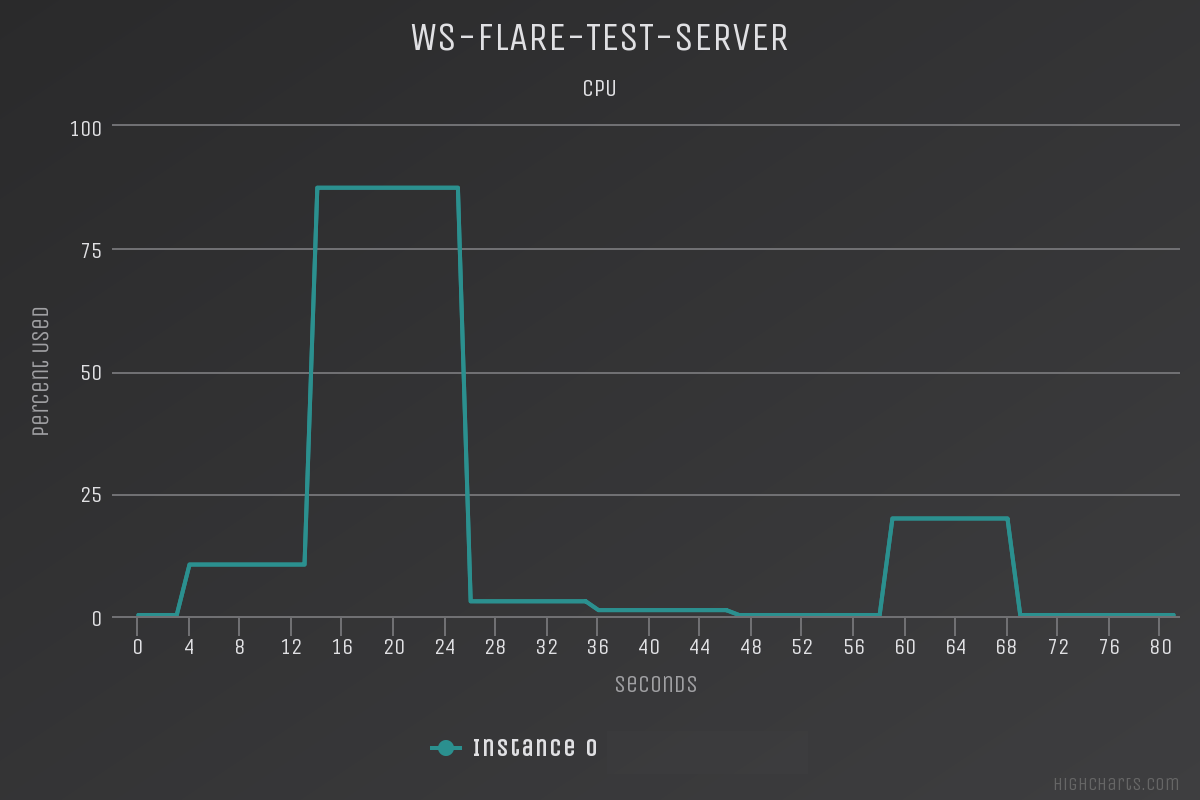
\includegraphics[width=0.8\textwidth]{figures/experiments/experiment-1/node-js/cpu-5000-256-memory.png}
    \caption{CPU consumption of websocket server testing 5000 connections with 256 MB of memory}
    \label{fig:experiment-1-cpu-5000-1-instances-256-mem}
\end{figure}

Comparing the CPU between using 4 instances of 64 MB of memory each in figure \ref{fig:experiment-1-cpu-5000-4-instances} with 1 instance and 256 MB of memory in figure \ref{fig:experiment-1-cpu-5000-1-instances-256-mem} it is clear that 1 instance yields 87\% memory consumption when connections were being established. However, with 4 instances, the CPU usage reached a maximum of 19\% per instance. This is due to the load balancing in effect here. Due to this, it can be concluded that using 4 instances instead of 1 will contribute to a more stable environment. 

\subsubsection{Simulating 30000 Connections}

For the next experiment, 30000 connections was attempted. Using the script in listing \ref{listing:nodejs-server-experiment-3}.

\begin{listing}[H]
    \caption{WS-Flare test script for simulating 30000 users}
    \label{listing:nodejs-server-experiment-3}
    \begin{minted}{json}
[
    {
        "start": 0,
        "timeout": 60,
        "totalSimulators": 30000,
        "target": "wss://ws-flare-test-server.cfapps.io:4443"
    }
]
\end{minted}
\end{listing}

There is 1 instance which is assigned a maximum of 2GB of memory as outlined in table \ref{table:cf-resource-limits-4}

\begin{table}[H]
\resizebox{0.7\textwidth}{!}{%
\begin{tabular}{ll}
\rowcolor[HTML]{ECF4FF} 
Instances & Memory Limit Per Instance \\
1         & 2GB     \\ 
\end{tabular}%
}
\caption{Cloud Foundry Resource Limits}
\label{table:cf-resource-limits-4}
\end{table}

\begin{figure}[H]
  \centering
    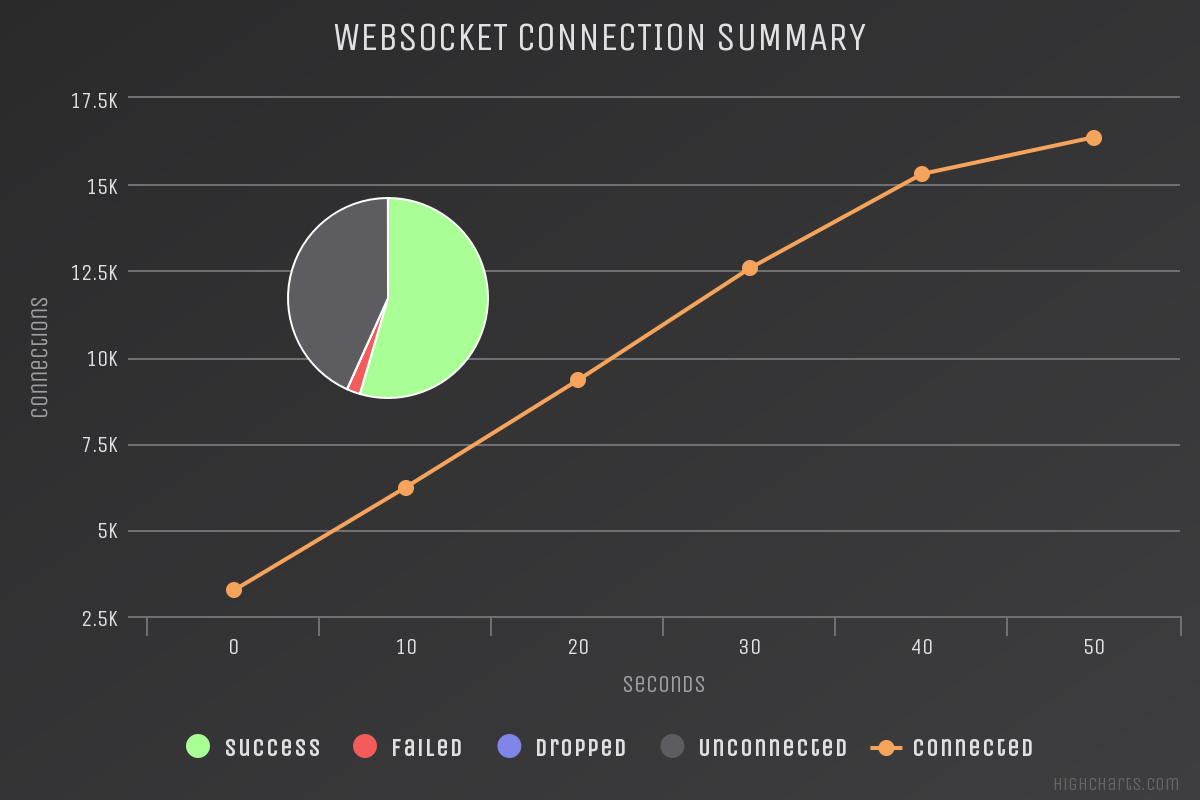
\includegraphics[width=0.8\textwidth]{figures/experiments/experiment-1/node-js/conn-summary-30000-256-memory.png}
    \caption{Results of simulating 30000 websockets with 256 MB of memory}
    \label{fig:experiment-3-conn-summary-5000-1-instances-256-mem}
\end{figure}

\begin{figure}[H]
  \centering
    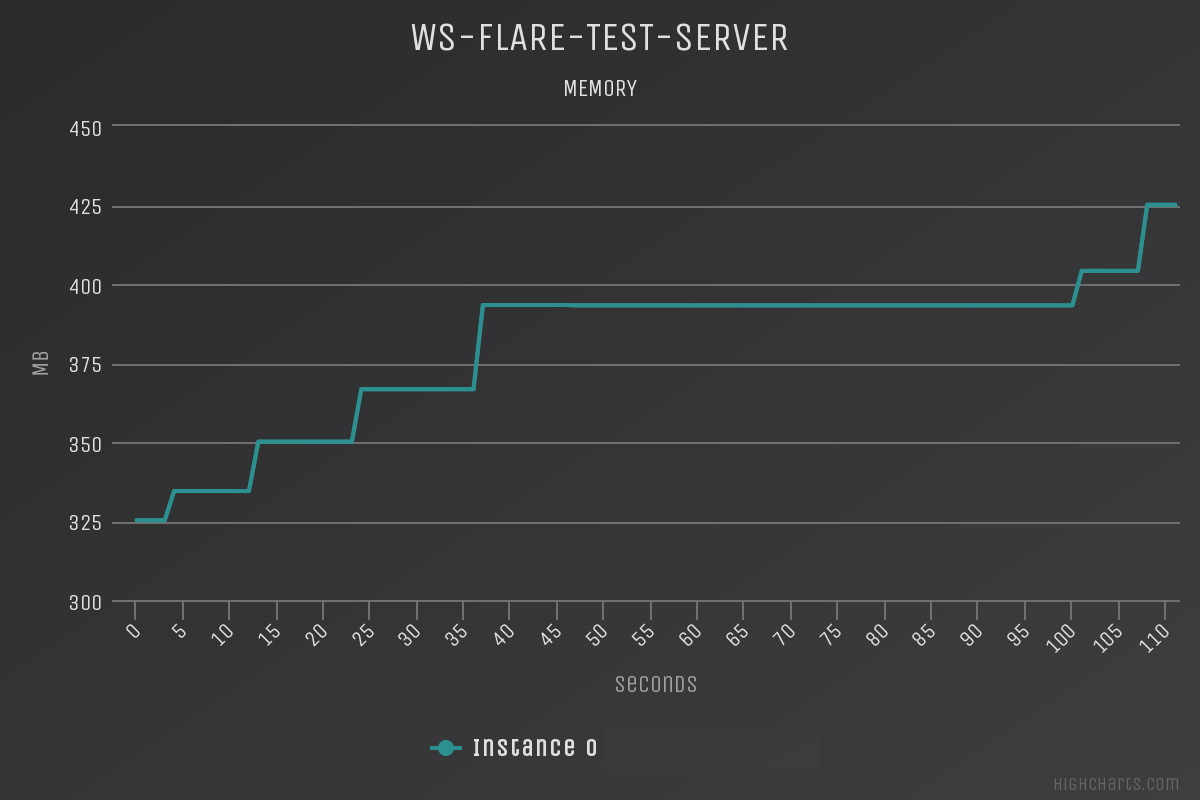
\includegraphics[width=0.8\textwidth]{figures/experiments/experiment-1/node-js/memory-30000-256-memory.png}
    \caption{Memory consumption of websocket server testing 30000 connections with 256 MB of memory}
    \label{fig:experiment-3-memory-5000-1-instances-256-mem}
\end{figure}

\begin{figure}[H]
  \centering
    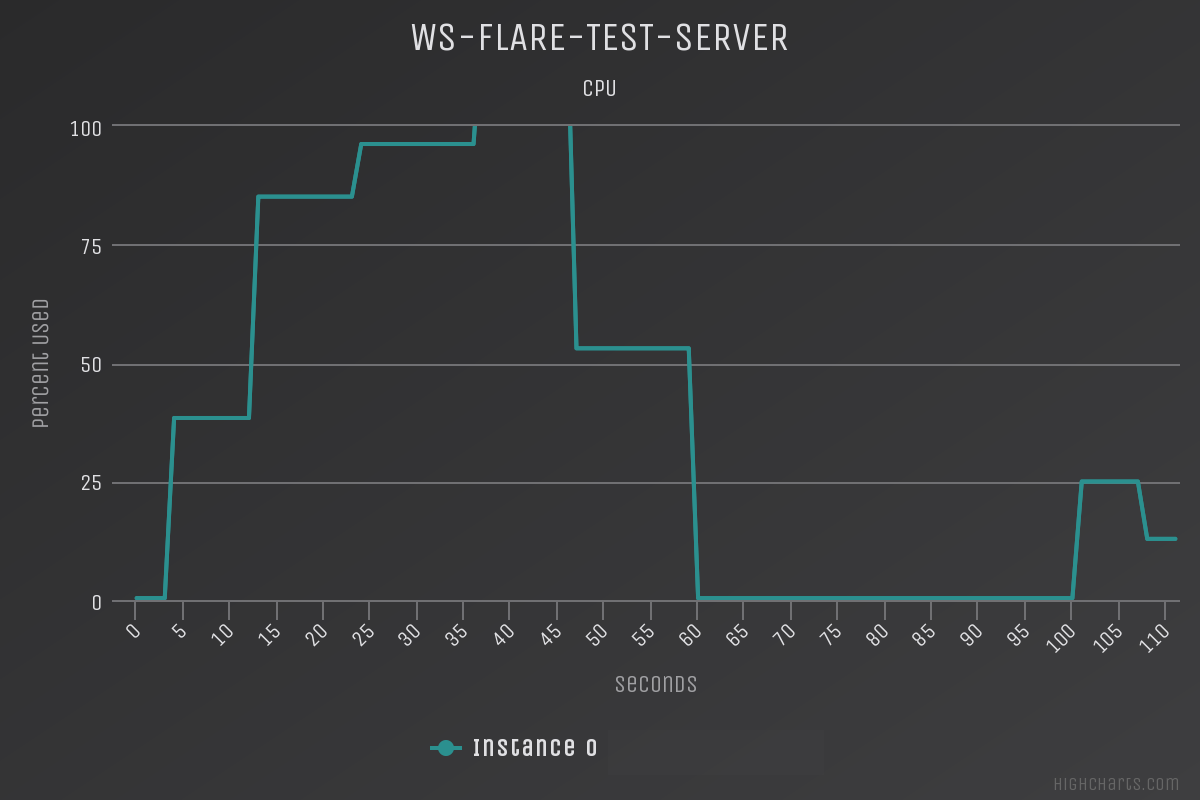
\includegraphics[width=0.8\textwidth]{figures/experiments/experiment-1/node-js/cpu-30000-256-memory.png}
    \caption{CPU consumption of websocket server testing 30000 connections with 256 MB of memory}
    \label{fig:experiment-3-cpu-5000-1-instances-256-mem}
\end{figure}

In figure \ref{fig:experiment-3-conn-summary-5000-1-instances-256-mem} it can be seen that the intended target of 30000 connections could not be reached. Instead, 16365 connections was achieved. The reason for this becomes clear when we look at figure  \ref{fig:experiment-3-cpu-5000-1-instances-256-mem}. 35 seconds into the test the CPU spiked to 120\% which goes over the 100\% limit imposed by Cloud Foundry. It is clear that a single server is not enough to allow 30000 connections. We can keep adding more and more memory, however, we are bound by the constraints of the CPU on Cloud Foundry, which means adding more memory would not achieve better results. Scaling to the resources defined in table \ref{table:cf-resource-limits-5} produced better results as can be seen in figure \ref{fig:experiment-3-conn-summary-30000-5-instances-512-mem}. There were 27764 successful connections and 2236 dropped connections.

\begin{table}[H]
\resizebox{0.7\textwidth}{!}{%
\begin{tabular}{ll}
\rowcolor[HTML]{ECF4FF} 
Instances & Memory Limit Per Instance \\
5         & 512MB     \\ 
\end{tabular}%
}
\caption{Cloud Foundry Resource Limits}
\label{table:cf-resource-limits-5}
\end{table}

\begin{figure}[H]
  \centering
    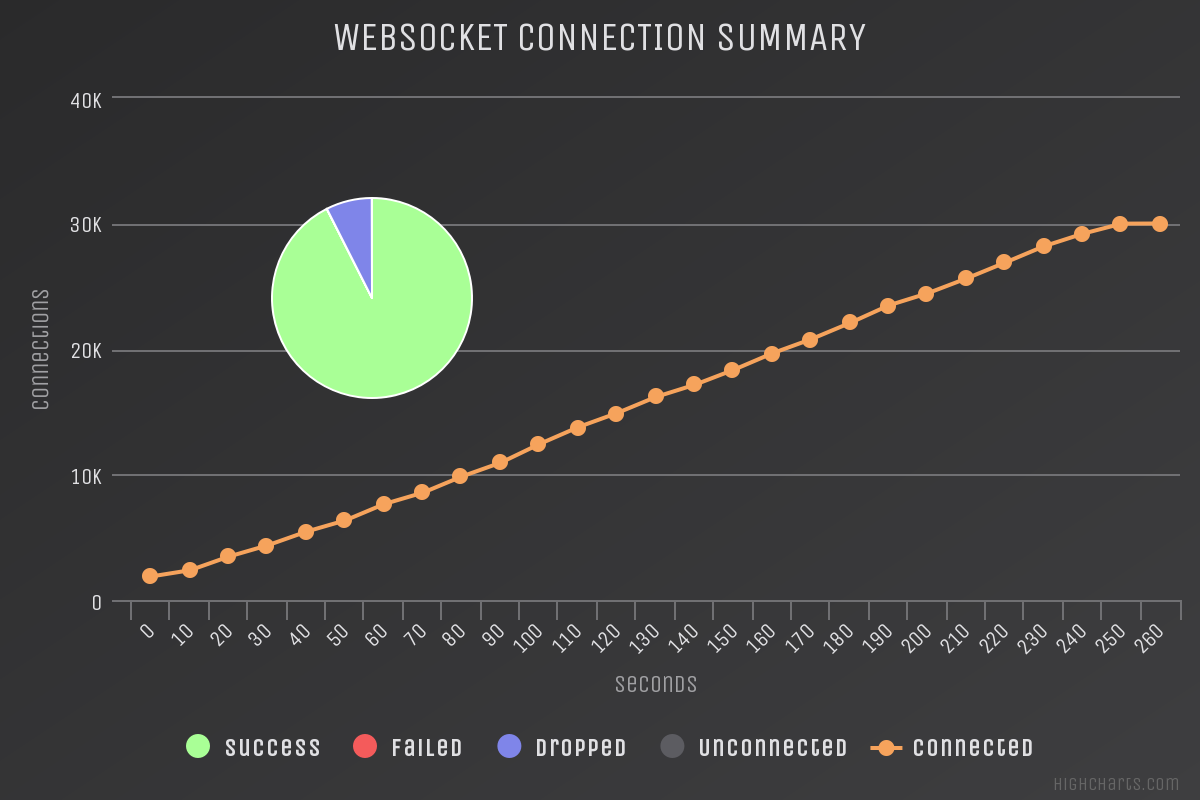
\includegraphics[width=0.8\textwidth]{figures/experiments/experiment-1/node-js/conn-summary-30000-5-instances-512-memory.png}
    \caption{Results of simulating 30000 websockets with 5 instances and 512 MB of memory}
    \label{fig:experiment-3-conn-summary-30000-5-instances-512-mem}
\end{figure}

\begin{figure}[H]
  \centering
    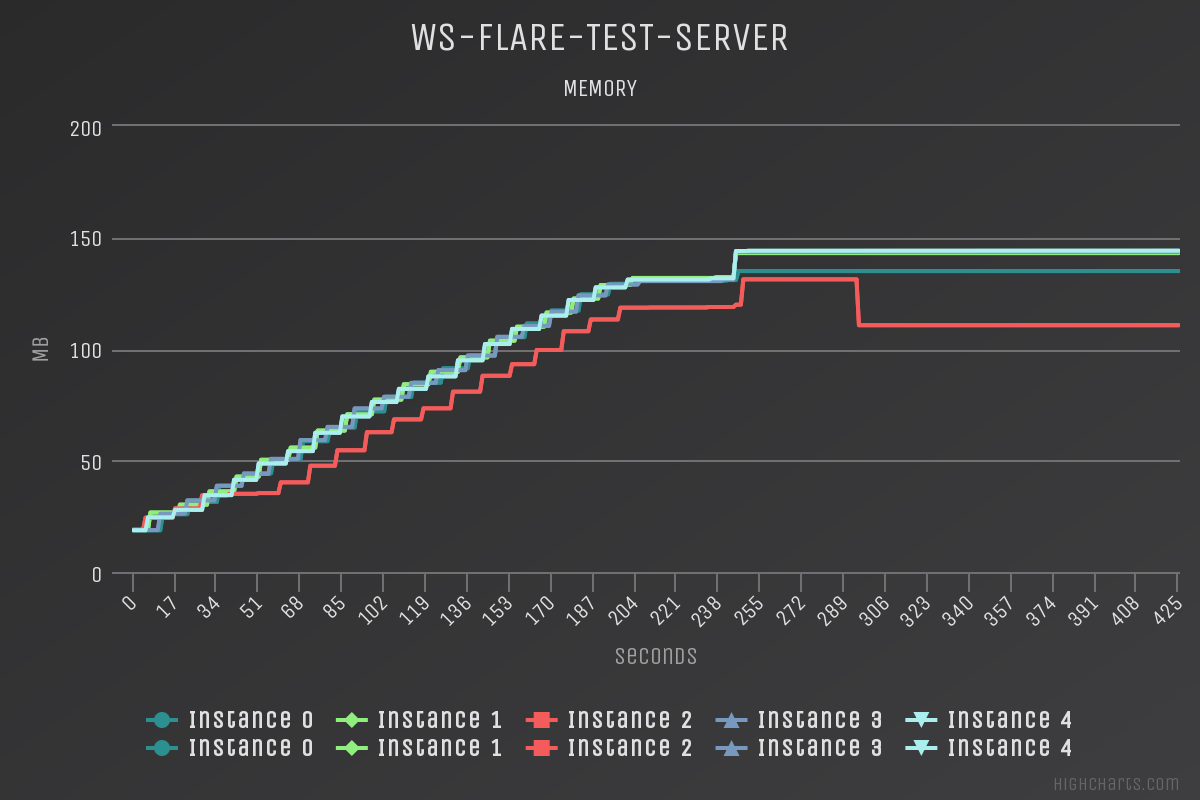
\includegraphics[width=0.8\textwidth]{figures/experiments/experiment-1/node-js/memory-30000-5-instances-512-memory.png}
    \caption{Memory consumption of websocket server testing 30000 connections with 5 instances and 512 MB of memory}
    \label{fig:experiment-3-memory-30000-5-instances-512-mem}
\end{figure}

\begin{figure}[H]
  \centering
    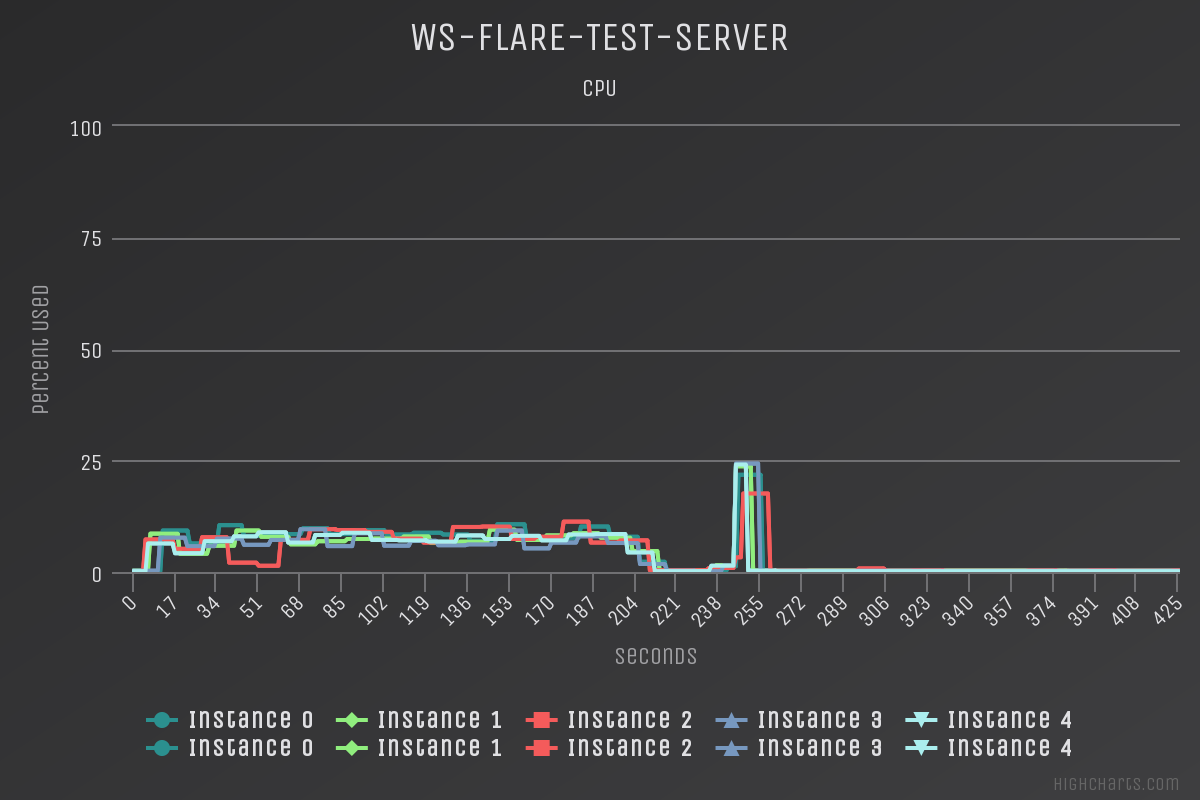
\includegraphics[width=0.8\textwidth]{figures/experiments/experiment-1/node-js/cpu-30000-5-instances-512-memory.png}
    \caption{CPU consumption of websocket server testing 30000 connections with 5 instances and 512 MB of memory}
    \label{fig:experiment-3-cpu-530000000-5-instances-512-mem}
\end{figure}

\subsection{GoLang WebSocket Server}

To test a GoLang server we wrote a small application using a library called gorilla web socket. The code for this can be seen in listing \ref{listing:golang-server-experiment-1}

\begin{listing}[H]
    \caption{GoLang Websocket Server Implementation}
    \label{listing:golang-server-experiment-1}
    \begin{minted}{go}
package main

import (
    "flag"
    "log"
    "net/http"

    "github.com/gorilla/websocket"
)

var addr = flag.String("addr", "0.0.0.0:8080", "http service address")

var upgrader = websocket.Upgrader{} // use default options

func echo(w http.ResponseWriter, r *http.Request) {
    c, err := upgrader.Upgrade(w, r, nil)
    if err != nil {
        log.Print("upgrade:", err)
        return
    }
    defer c.Close()
    for {
        mt, message, err := c.ReadMessage()
        if err != nil {
            log.Println("read:", err)
            break
        }
        log.Printf("recv: %s", message)
        err = c.WriteMessage(mt, message)
        if err != nil {
            log.Println("write:", err)
            break
        }
    }
}

func main() {
    flag.Parse()
    log.SetFlags(0)
    http.HandleFunc("/echo", echo)
    log.Fatal(http.ListenAndServe(*addr, nil))
}
\end{minted}
\end{listing}

\subsubsection{Simulating 1000 connections}

\begin{table}[H]
\resizebox{0.7\textwidth}{!}{%
\begin{tabular}{ll}
\rowcolor[HTML]{ECF4FF} 
Instances & Memory Limit Per Instance \\
1         & 64MB     \\ 
\end{tabular}%
}
\caption{Cloud Foundry Resource Limits}
\label{table:cf-resource-golang-1000-64}
\end{table}

\begin{figure}[H]
  \centering
    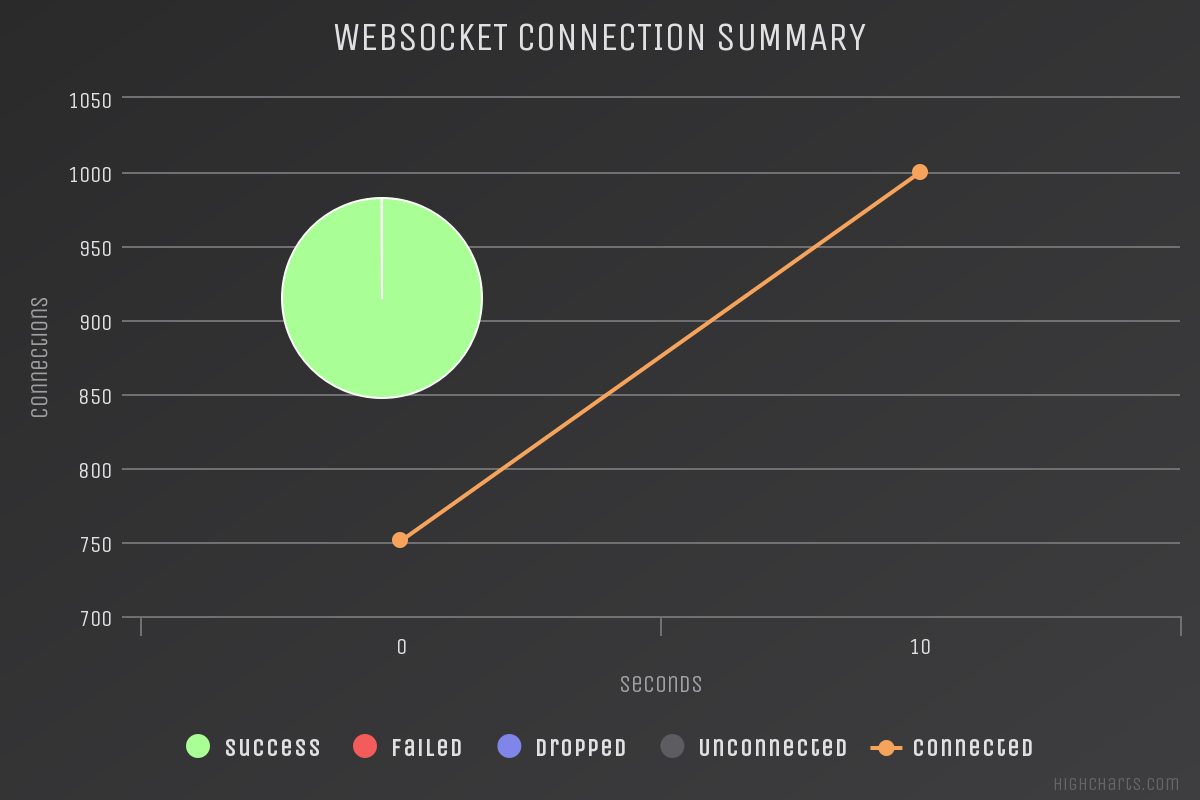
\includegraphics[width=0.8\textwidth]{figures/experiments/experiment-1/golang/conn-1000-64-memory.png}
    \caption{Results of simulating 10000 websockets with 64 MB of memory using GoLang server}
    \label{fig:experiment-1-golang-conn-1000-64}
\end{figure}

\begin{figure}[H]
  \centering
    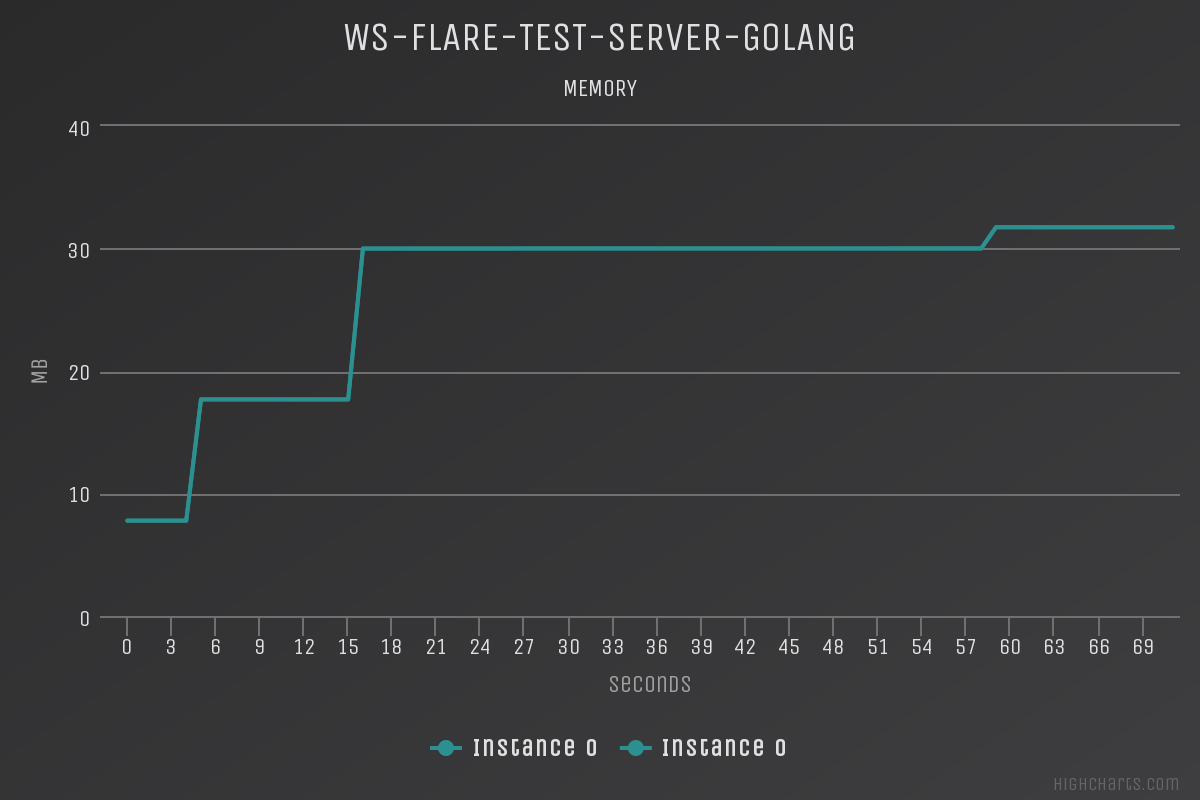
\includegraphics[width=0.8\textwidth]{figures/experiments/experiment-1/golang/memory-1000-64.png}
    \caption{Memory consumption of websocket server testing 1000 connections with 1 instances and 64 MB of memory using GoLang server}
    \label{fig:experiment-1-golang-memory-1000-64}
\end{figure}

\begin{figure}[H]
  \centering
    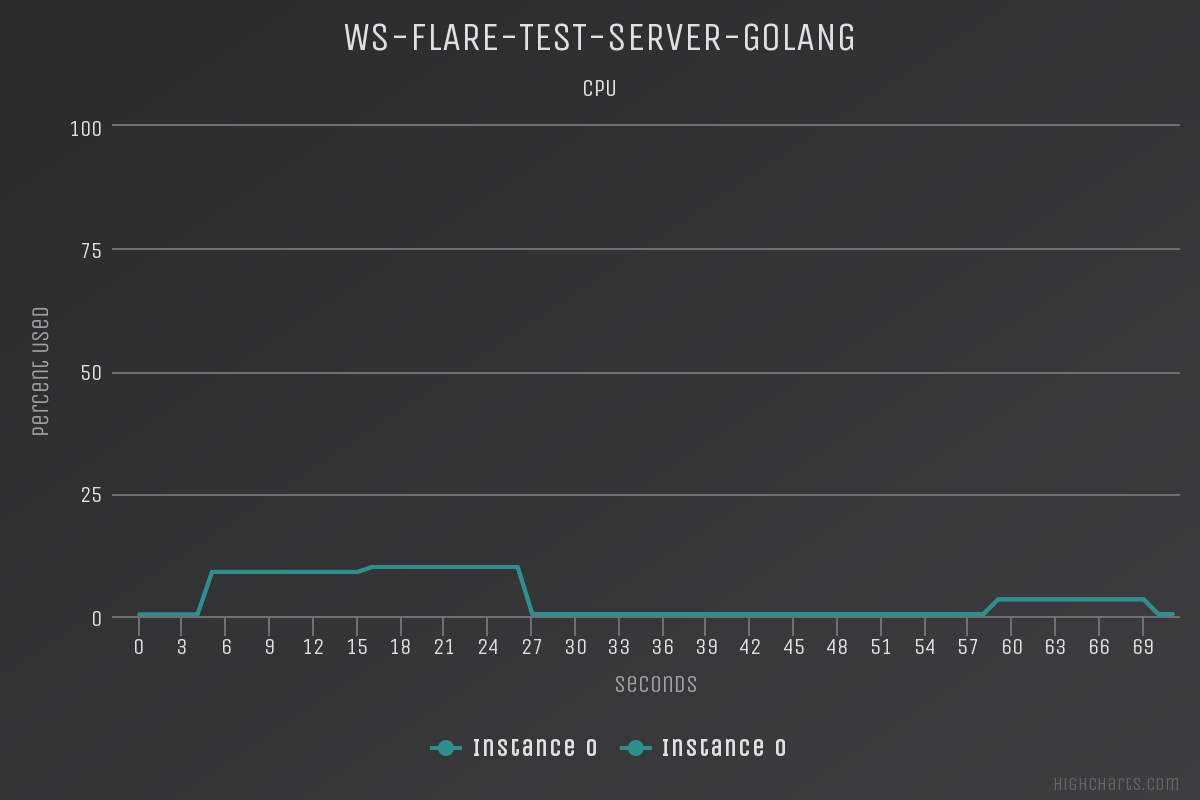
\includegraphics[width=0.8\textwidth]{figures/experiments/experiment-1/golang/cpu-1000-64.png}
    \caption{CPU consumption of websocket server testing 1000 connections with 1 instances and 64 MB of memory using GoLang server}
    \label{fig:experiment-1-golang-cpu-1000-64}
\end{figure}

Much like NodeJs, the GoLang server had no trouble handling 1000 simultaneous connections. It is worth noting however that the connections for NodeJs connected faster than with GoLang. Figure \ref{fig:experiment-1-node-conn-summary-1000} shows that all connections in less than 1 second while figure \ref{fig:experiment-1-golang-conn-1000-64} shows that it took 10 seconds longer for all 1000 connections to connect when using GoLang.

\subsubsection{Simulating 5000 connections}

Through experimentation we found that either of the resources defined in table \ref{table:cf-resource-golang-5000} were needed in order to reach 5000 simultaneous connections.

\begin{table}[H]
\resizebox{0.7\textwidth}{!}{%
\begin{tabular}{ll}
\rowcolor[HTML]{ECF4FF} 
Instances & Memory Limit Per Instance \\
3         & 64MB     \\ 
1         & 256MB
\end{tabular}%
}
\caption{Cloud Foundry Resource Limits}
\label{table:cf-resource-golang-5000}
\end{table}

For a single instance, this remains the same as what we saw for NodeJs in table \ref{table:cf-resource-limits-3}. However, for multiple instances, we see that we can use one less instance than NodeJs. 

\subsubsection{Simulating 30000 connections}

Reaching 30000 connections to a GoLang web socket server could not be achieved. The resources in \ref{table:cf-resource-golang-30000} were used. However, the most that could be achieved was 26000 connections. And a lot of these connections dropped after a few seconds as can be seen in figure \ref{fig:experiment-1-golang-conn-30000-512-10}. NodeJs performed better when simulating 30000 connections. This seems to suggest that GoLang web sockets perform better when there are fewer connections however the performance degrades as more connections are added. Figure \ref{fig:experiment-1-golang-cpu-30000-512-10} also suggests that CPU for the GoLang web server remains stable no matter how many connections there are.

\begin{table}[H]
\resizebox{0.7\textwidth}{!}{%
\begin{tabular}{ll}
\rowcolor[HTML]{ECF4FF} 
Instances & Memory Limit Per Instance \\
10         & 512MB     \\
\end{tabular}%
}
\caption{Cloud Foundry Resource Limits}
\label{table:cf-resource-golang-30000}
\end{table}

\begin{figure}[H]
  \centering
    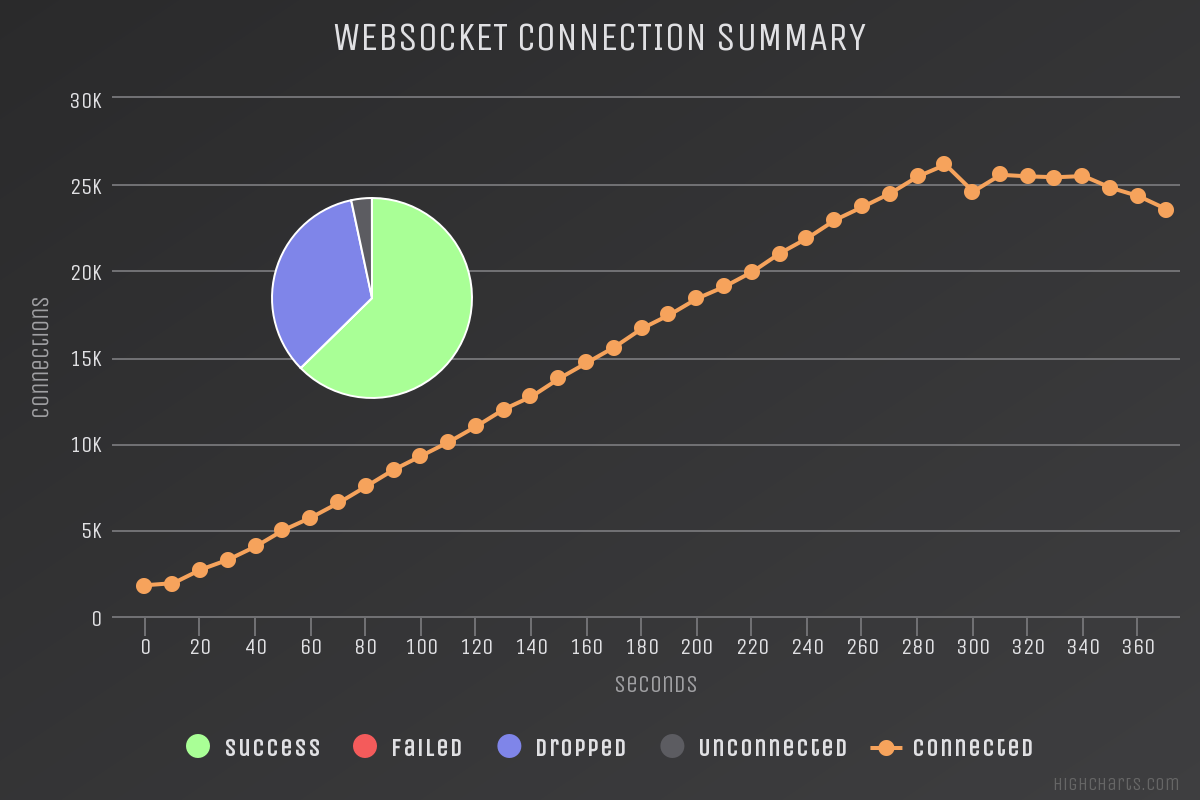
\includegraphics[width=0.8\textwidth]{figures/experiments/experiment-1/golang/conn-30000-512-10.png}
    \caption{Results of simulating 30000 websockets with 10 instances and 512 MB of memory using GoLang server}
    \label{fig:experiment-1-golang-conn-30000-512-10}
\end{figure}

\begin{figure}[H]
  \centering
    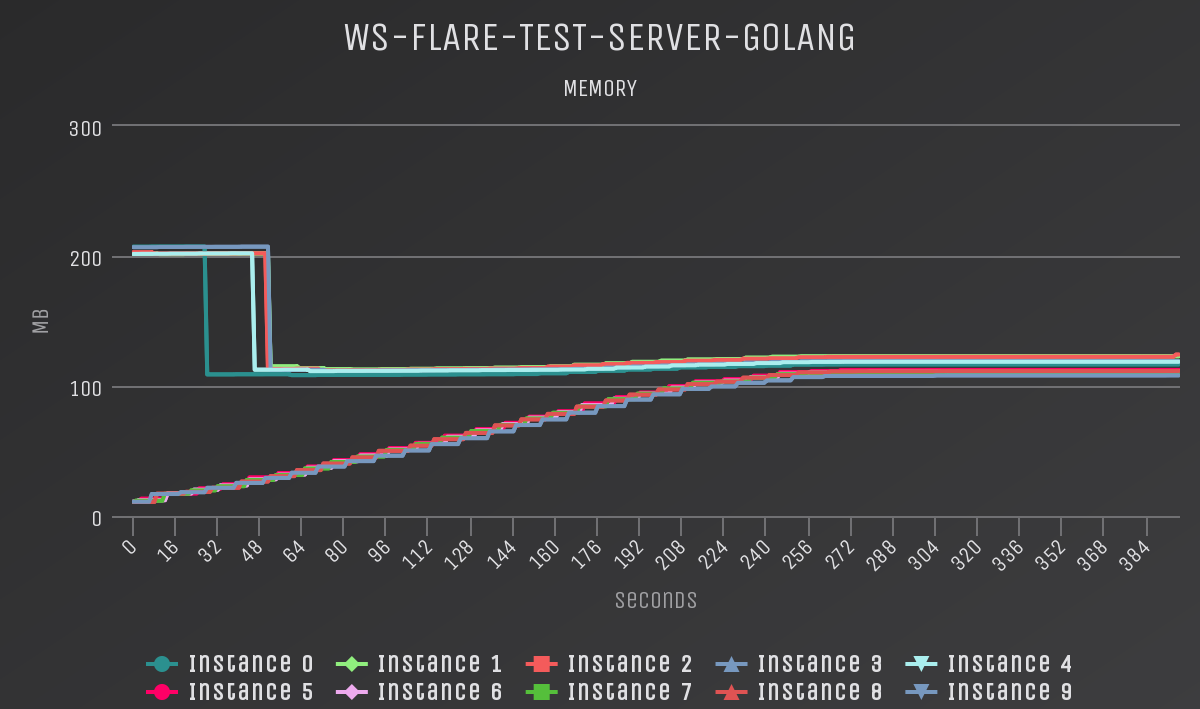
\includegraphics[width=0.8\textwidth]{figures/experiments/experiment-1/golang/memory-30000-512-10.png}
    \caption{Memory consumption of websocket server testing 1000 connections with 10 instances and 512 MB of memory using GoLang server}
    \label{fig:experiment-1-golang-memory-30000-512-10}
\end{figure}

\begin{figure}[H]
  \centering
    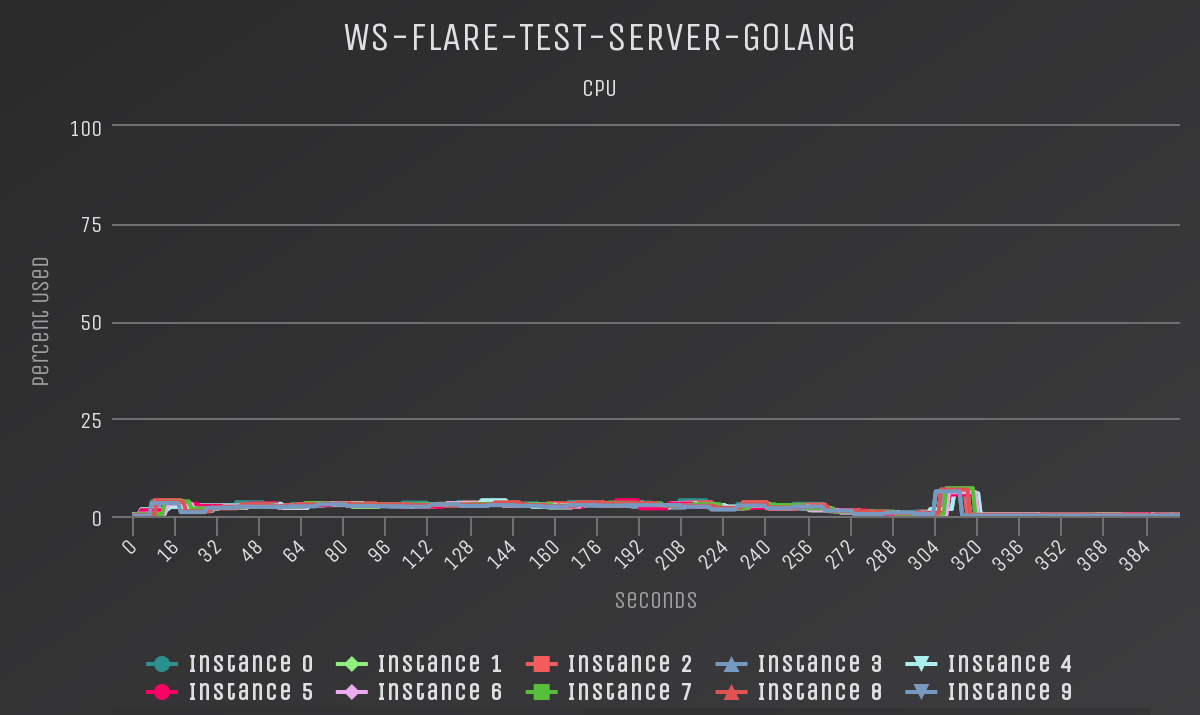
\includegraphics[width=0.8\textwidth]{figures/experiments/experiment-1/golang/cpu-30000-512-10.png}
    \caption{CPU consumption of websocket server testing 30000 connections with 10 instances and 512 MB of memory using GoLang server}
    \label{fig:experiment-1-golang-cpu-30000-512-10}
\end{figure}

\section{Testing Backend With Multiple Services}

To test the ability to monitor multiple services at the same time using the ws-flare framework, we created 3 microservices written in NodeJS. The first microservice is a web socket server as shown in listing \ref{listing:experiment-2-cluster-websocket-server}. This service will accept web socket connections, once a connection has been made it will then send a request to service 1 which is outlined in listing \ref{listing:experiment-2-service-1} every 5 seconds until the connection is closed. Service 1 will send a request to service 2 which is defined in listing \ref{listing:experiment-2-service-2}. Service 2 will respond with a hello message and a number counter which will increment after every request.

\begin{listing}[H]
    \caption{Websocket Server}
    \label{listing:experiment-2-cluster-websocket-server}
    \begin{minted}{javascript}
const http = require('http');
const WebSocket = require('ws');
const superagent = require('superagent');

const server = http.createServer();
const wss = new WebSocket.Server({noServer: true});

wss.on('connection', (ws) => {
    console.log('new connection');

    const interval = setInterval(() => {
        superagent
            .get('https://ws-flare-cluster-service-1.cfapps.io/endpoint')
            .end((err, res) => {
                ws.send(JSON.stringify(res.body));
            });
    }, 5000);

    ws.on('close', () => {
        clearInterval(interval);
        console.log('connection dropped');
    });
});

server.on('upgrade', function upgrade(request, socket, head) {
    wss.handleUpgrade(request, socket, head, function done(ws) {
        wss.emit('connection', ws, request);
    });
});

server.listen(process.env.PORT || 3000, () => {
    console.log('Starting ws server');
});

\end{minted}
\end{listing}

\begin{listing}[H]
    \caption{Service 1}
    \label{listing:experiment-2-service-1}
    \begin{minted}{javascript}
const express = require('express');
const app = express();
const superagent = require('superagent');
const port = process.env.PORT || 3000;

app.get('/endpoint', (_, res) => {
    superagent
        .get('https://ws-flare-cluster-service-2.cfapps.io/endpoint')
        .end((_, response) => {
            res.json(response.body);
        });
});

app.listen(port, () => console.log('listening on port ' + port));
\end{minted}
\end{listing}

\begin{listing}[H]
    \caption{Service 2}
    \label{listing:experiment-2-service-2}
    \begin{minted}{javascript}
const express = require('express');
const app = express();
const port = process.env.PORT || 3000;

let counter = 0;

app.get('/endpoint', (req, res) => {
    counter++;
    res.json({message: 'Hello ' + counter});
});

app.listen(port, () => console.log('listening on port ' + port));
\end{minted}
\end{listing}

\begin{table}[H]
\resizebox{\textwidth}{!}{%
\begin{tabular}{lll}
\rowcolor[HTML]{ECF4FF} 
Name             & Instances & Memory Limit Per Instance \\
websocket-server & 15        & 512MB                     \\
service 1        & 15        & 256MB                     \\
service2         & 5         & 256MB                    
\end{tabular}%
}
\caption{Resources allocated to each service}
\label{table:cf-resource-experiment-2-10000}
\end{table}

\subsubsection{10000 connections}

In order to reach 10000 concurrent connections we had to use the resources defined in table \ref{table:cf-resource-experiment-2-10000}. The number of resources required here are substantial when we compare this to what the server is doing, this seems massively inflated, however, the results seem to indicate massive CPU usage in service 1 which seems to act as a bottleneck, as can be seen in figure \ref{fig:experiment-2-service-1-cpu-10000} some of the services go above the 100\% threshold for the CPU. Even with the substantial amount of resources assigned to each service we still see a lot of dropped connections as can be seen in figure \ref{fig:experiment-2-conn-10000}. The web socket service and service 2 appear to have operated better in this experiment as can be seen from figure \ref{fig:experiment-2-ws-cpu-10000} and figure \ref{fig:experiment-2-service-2-cpu-10000}, the CPU remained at reasonable levels well within the 100\% CPU threshold.

\begin{figure}[H]
  \centering
    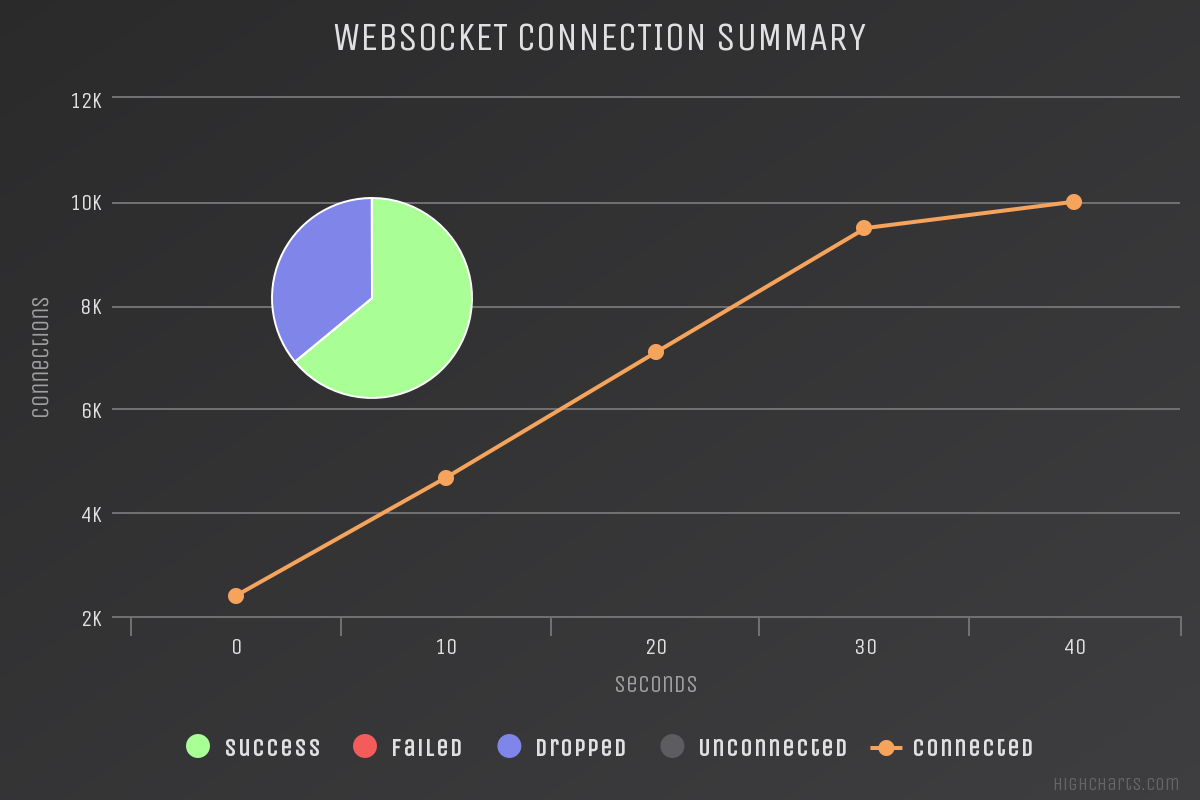
\includegraphics[width=0.8\textwidth]{figures/experiments/experiment-2/10000/conn-10000.png}
    \caption{Results of simulating 10000 websockets against 3 microservices}
    \label{fig:experiment-2-conn-10000}
\end{figure}

\begin{figure}[H]
  \centering
    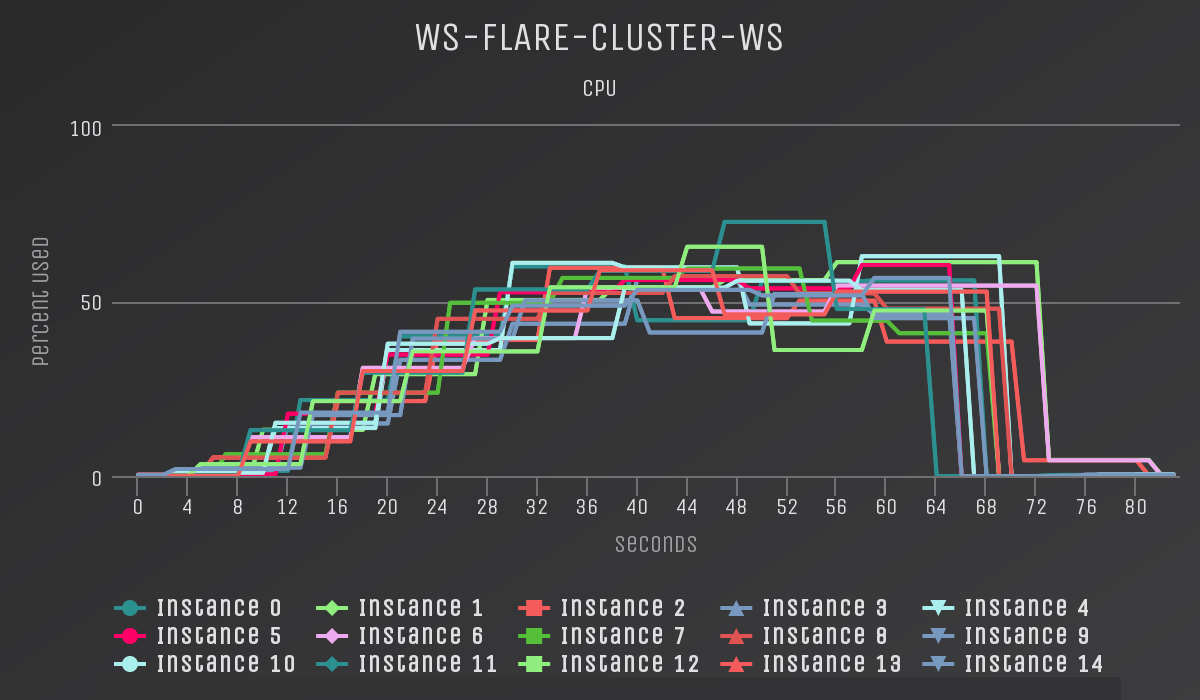
\includegraphics[width=0.8\textwidth]{figures/experiments/experiment-2/10000/ws-cpu-10000.png}
    \caption{WebSocket Server CPU usage}
    \label{fig:experiment-2-ws-cpu-10000}
\end{figure}

\begin{figure}[H]
  \centering
    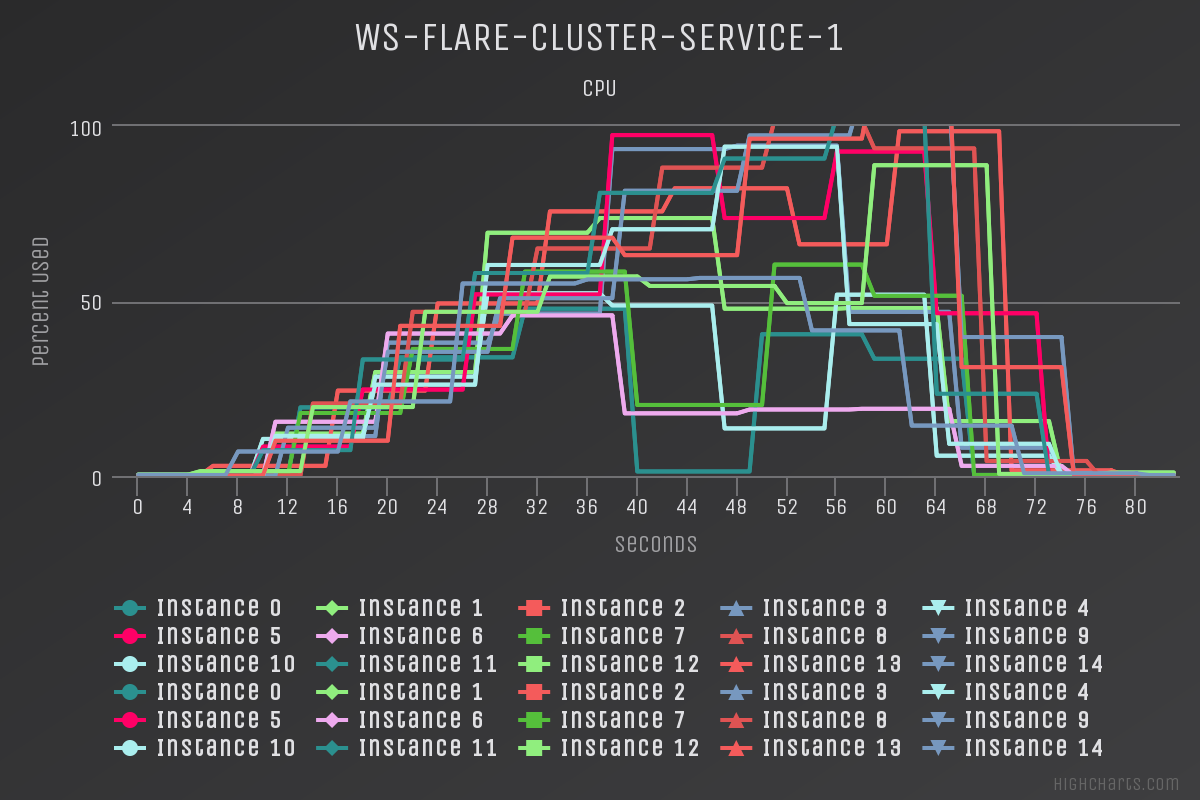
\includegraphics[width=0.8\textwidth]{figures/experiments/experiment-2/10000/service1-cpu-10000.png}
    \caption{Service 1 CPU usage}
    \label{fig:experiment-2-service-1-cpu-10000}
\end{figure}

\begin{figure}[H]
  \centering
    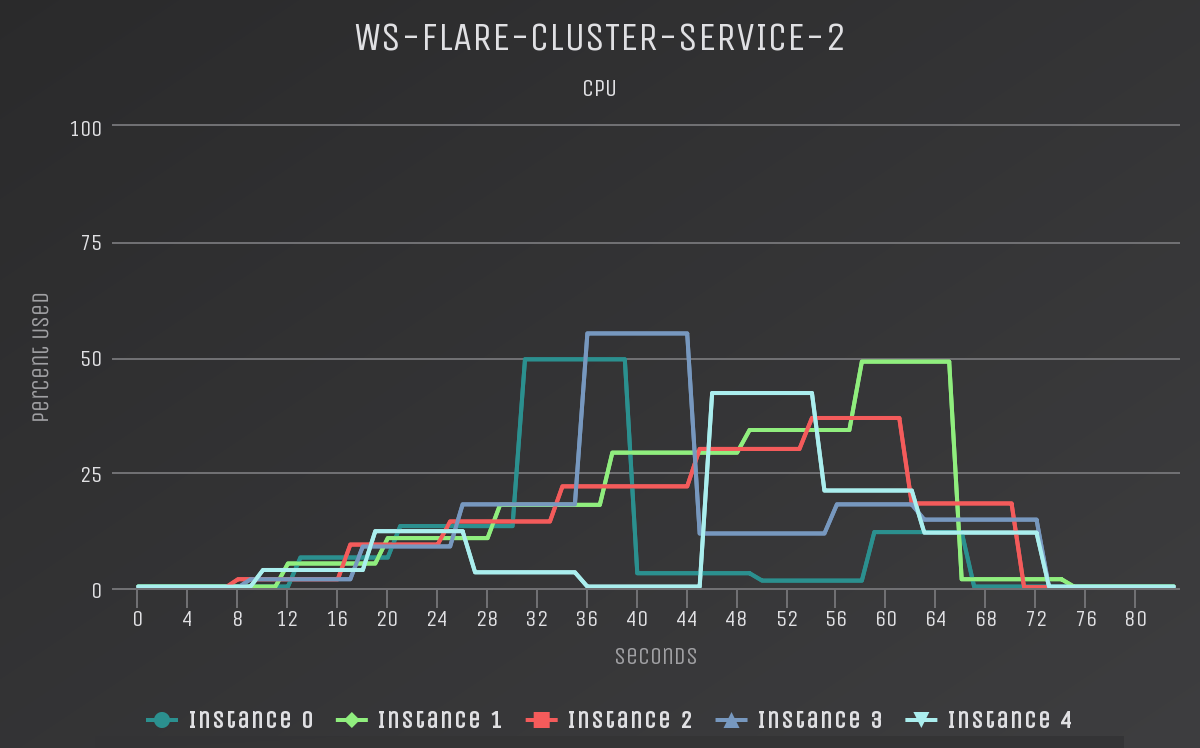
\includegraphics[width=0.8\textwidth]{figures/experiments/experiment-2/10000/service2-cpu-10000.png}
    \caption{Service 2 CPU usage}
    \label{fig:experiment-2-service-2-cpu-10000}
\end{figure}

From these results, it is clear that introducing any network related activity between services has a substantial impact on the performance of services deployed to Cloud Foundry.

\section{Usage in Continuous Integration}

With the ever growing shift from manual testing to automated testing there are a large number of tools available which can automate tasks seamless. TravisCI \cite{travisCI}, AppveyorCI \cite{appveyorCI} and Jenkins \cite{jenkinsCi} are some of the more popular tools available in this area. We wanted to test the integration between the ws-flare platform and continuous integration tools in order to demonstrate that this new platform can easily integrate with other tools. We created a command line tool that could integrate with the ws-flare platform. The command line tool is named ws-flare-cli. The tool is distributed as an NPM package and can be installed on any system that is running NodeJS. To install the package the command in listing \ref{listing:ws-flare-cli-install} can be used. This makes the CLI tool available to use in a command prompt.

\begin{listing}[H]
    \caption{Command to install the ws-flare-cli package}
    \label{listing:ws-flare-cli-install}
    \begin{minted}{bash}
npm install -g ws-flare-cli
\end{minted}
\end{listing}

The tool takes 2 parameters as demonstrated in listing \ref{listing:ws-flare-cli-parameters-example}. The first parameters is the URL to where the ws-flare platform is located. The second parameter is the generated token needed to gain access to to the GraphQL interface. This token is encrypted with JWT (JSON Web Token) for security reasons. If the wrong token is provided then the ws-flare platform will reject the request to start a task.

\begin{listing}[H]
    \caption{Command to run a task on the ws-flare platform}
    \label{listing:ws-flare-cli-parameters-example}
    \begin{minted}{bash}
ws-flare-cli --server=<WS-FLARE-SERVER-LOCATION> --token=<TASK-TOKEN>
\end{minted}
\end{listing}

To demonstrate that the ws-flare-cli tool can be easily integrated into multiple continuous integration tools, we created 2 experiments. The first uses TravisCI and the second uses AppveyorCI. Travis reads commands from a file called ``.travis.yml``. The file contents are shown in listing \ref{listing:ws-flare-cli-travis-yaml}

\begin{listing}[H]
    \caption{Travis YAML file for running ws-flare-cli commands}
    \label{listing:ws-flare-cli-travis-yaml}
    \begin{minted}{yaml}
language: node_js
node_js:
  - '8'
install:
  - npm i -g ws-flare-cli
script:
  - ws-flare-cli 
  --server=http://34.95.74.250 
  --token=eyJhbGciOiJIUzI1NiIsInR5cCI6IkpXVCJ9
  \ .eyJ1c2VySWQiOiJiMmI3MDA1ZC0xNmQ1LTQ2YzEtOTQ
  \ xNy1kMzYzMzY5ZDI4OTkiLCJ0YXNrSWQiOiI3MzU2Mz
  \ cwOC03NzRiLTQyM2EtYjE5MC0xMzEzNWM4NTk4ZTUiL
  \ CJpYXQiOjE1NTc2NTQ5NDEsImV4cCI6MTU4OTE5MDk0MX0
  \ .Gf5RLHlEw5paJFrzI0mFdKgUzNc1S3M3SAgN-wMR1Nw
\end{minted}
\end{listing}

\begin{figure}[H]
  \centering
    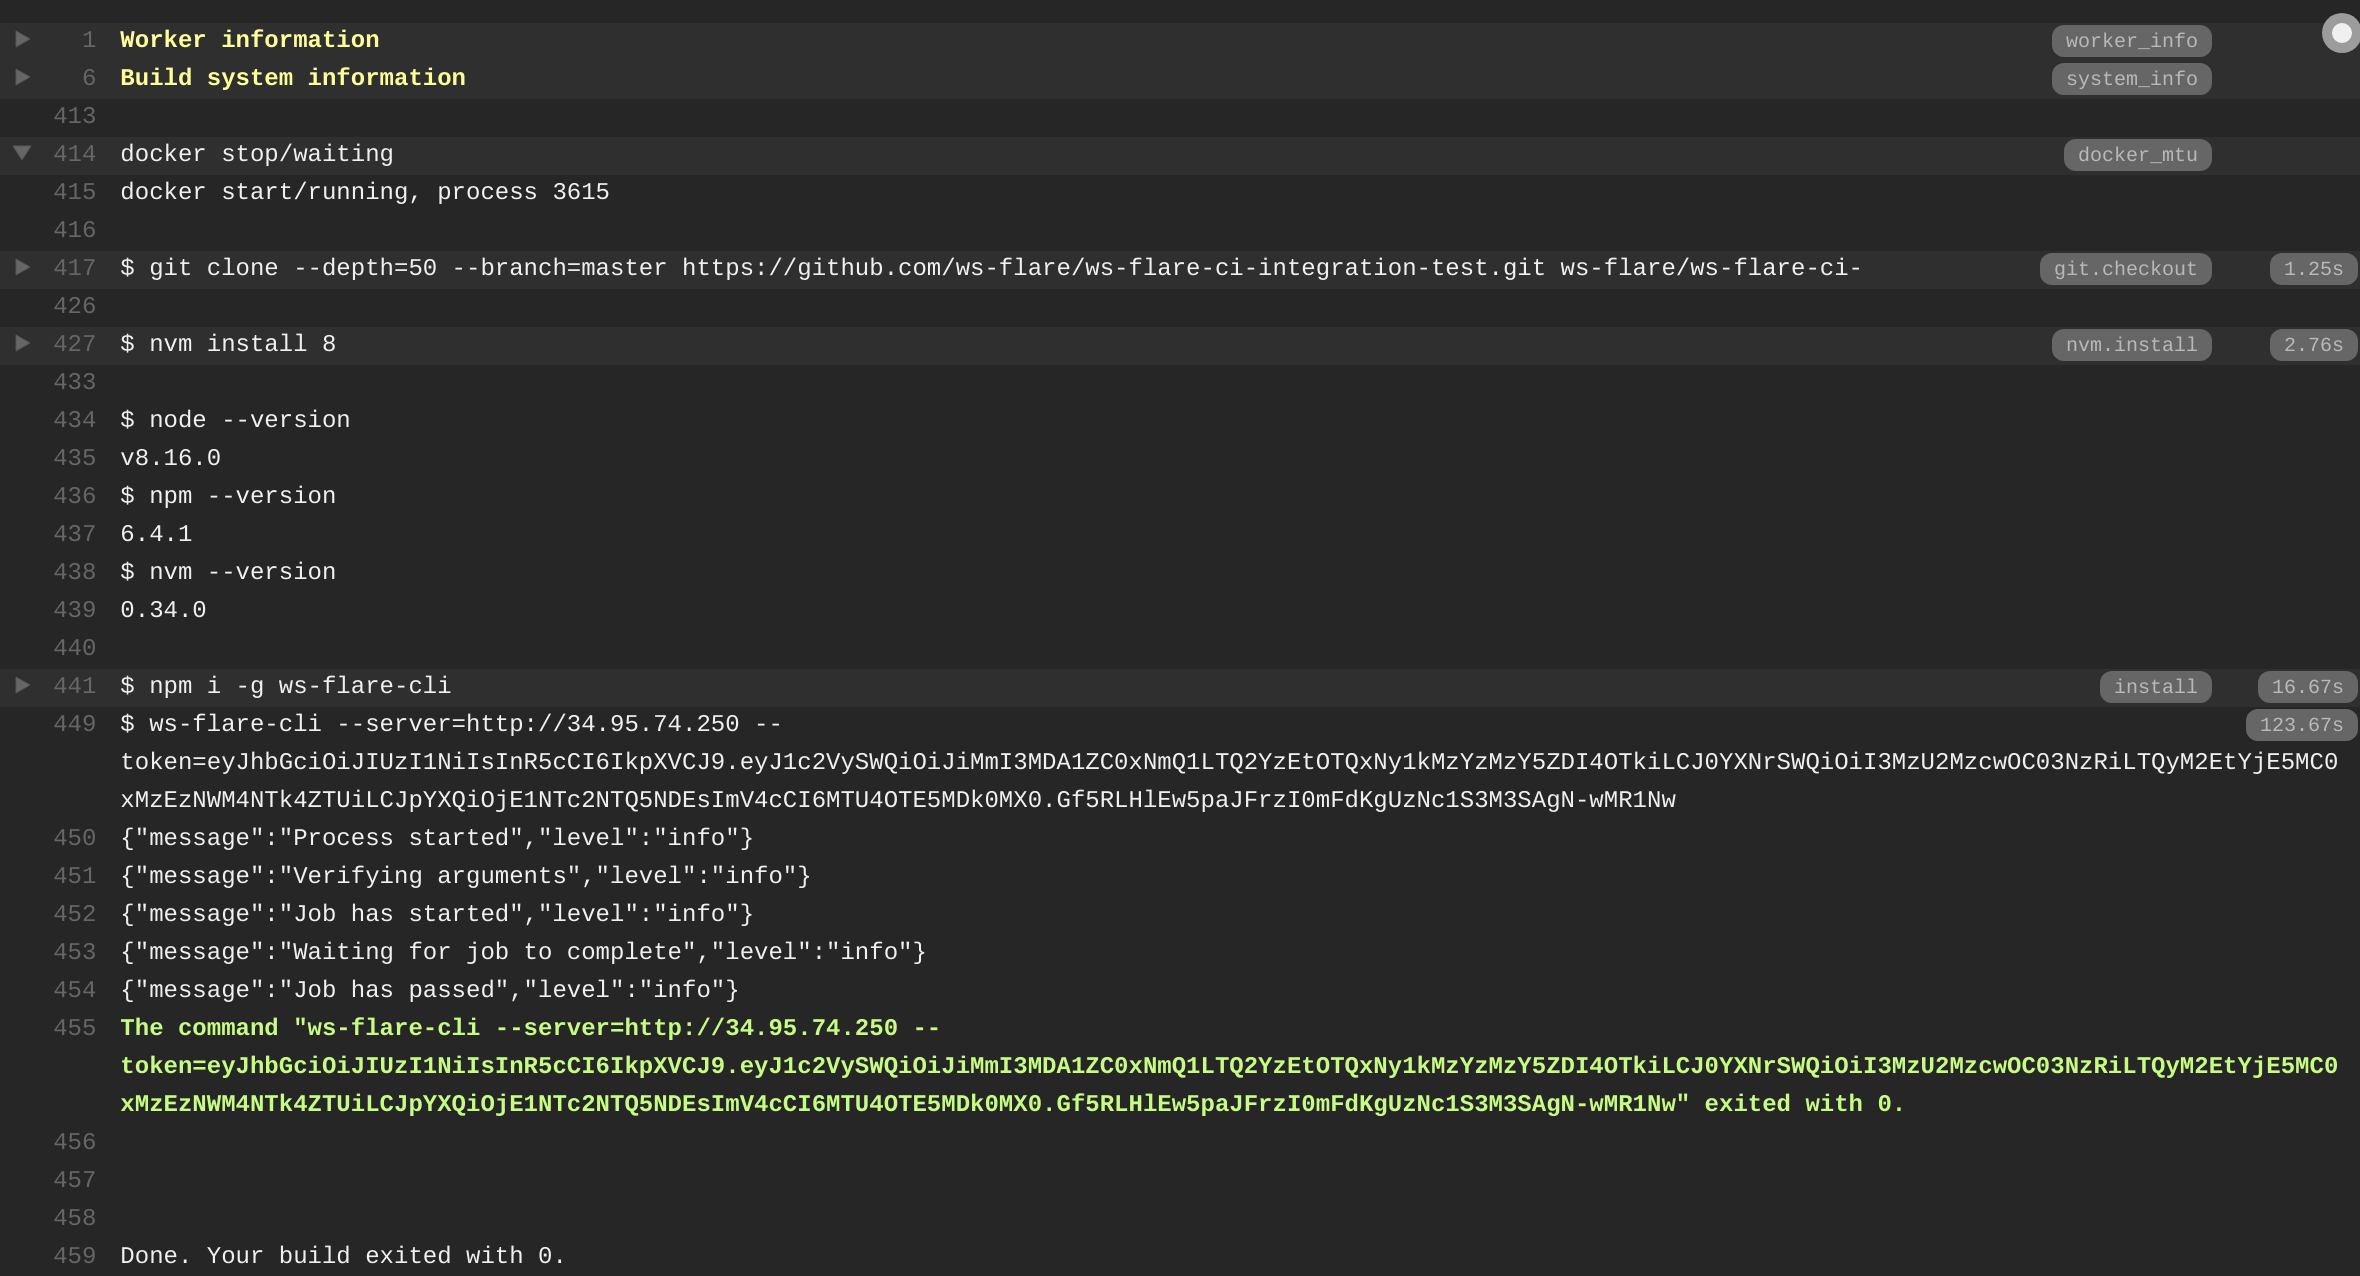
\includegraphics[width=1\textwidth]{figures/experiments/experiment-3/travis-output.png}
    \caption{TravisCI log output for running ws-flare-cli command}
    \label{fig:experiment-3-travis-log}
\end{figure}

As can be seen in figure \ref{fig:experiment-3-travis-log}, the command line tool was installed and then the tool communicated with the ws-flare platform at the specified address and ran a test against a web socket server. The result, in this case, was the build passed. If however, the test failed it would fail the Travis build. 

Similar to Travis Appveyor uses a YAML file called ``appveyor.yml``. The contents of this file can be seen in listing \ref{listing:ws-flare-cli-appveyor-yaml}

\begin{listing}[H]
    \caption{AppveyorCI YAML file for running ws-flare-cli commands}
    \label{listing:ws-flare-cli-appveyor-yaml}
    \begin{minted}{yaml}
os: Visual Studio 2015

environment:
  nodejs_version: "8"

install:
  - ps: Install-Product node env:nodejs_version
  - npm i -g ws-flare-cli

test_script:
  - ws-flare-cli --server=http://34.95.74.250 
  --token=eyJhbGciOiJIUzI1NiIsInR5cCI6IkpXVCJ9
  \ .eyJ1c2VySWQiOiJiMmI3MDA1ZC0xNmQ1LTQ2YzEtO
  \ TQxNy1kMzYzMzY5ZDI4OTkiLCJ0YXNrSWQiOiI3MzU2M
  \ zcwOC03NzRiLTQyM2EtYjE5MC0xMzEzNWM4NTk4ZTUiL
  \ CJpYXQiOjE1NTc2NTQ5NDEsImV4cCI6MTU4OTE5MDk0MX
  \ 0.Gf5RLHlEw5paJFrzI0mFdKgUzNc1S3M3SAgN-wMR1Nw

build: off
\end{minted}
\end{listing}

The corresponding output from running against Appveyor can be seen in listing \ref{fig:experiment-3-appveyor-log}. In this experiment, the test passed again, however it failed it would also fail the build as demonstrated in figure \ref{fig:experiment-3-appveyor-log-failed}. Failing the build is as important as passing the build. If the build fails it will prevent the code from being merged that could impact the performance of the system.

\begin{figure}[H]
  \centering
    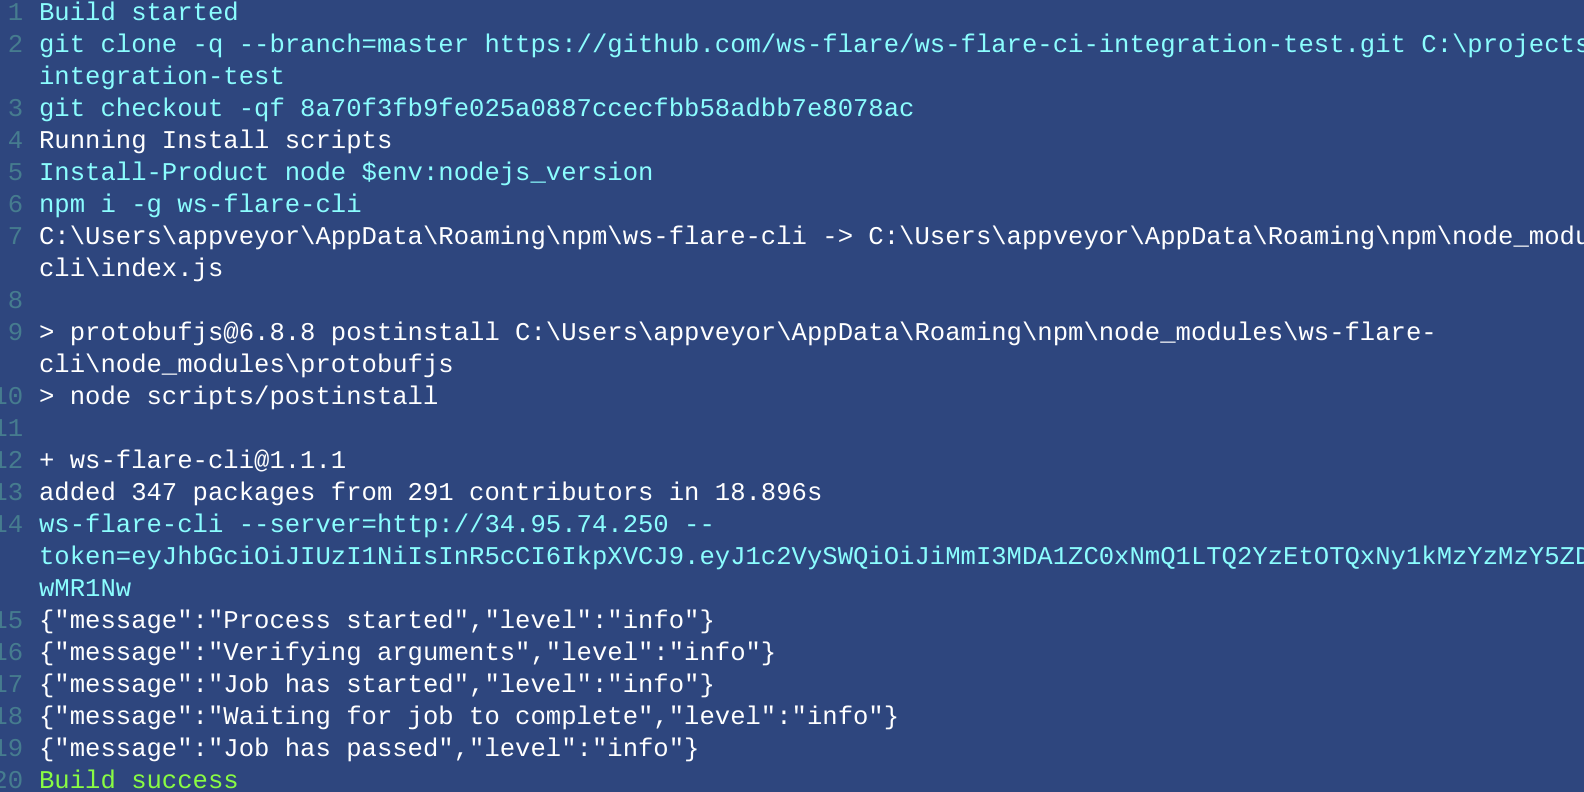
\includegraphics[width=1\textwidth]{figures/experiments/experiment-3/appveyor-output.png}
    \caption{Appveryor log output for running ws-flare-cli command}
    \label{fig:experiment-3-appveyor-log}
\end{figure}

\begin{figure}[H]
  \centering
    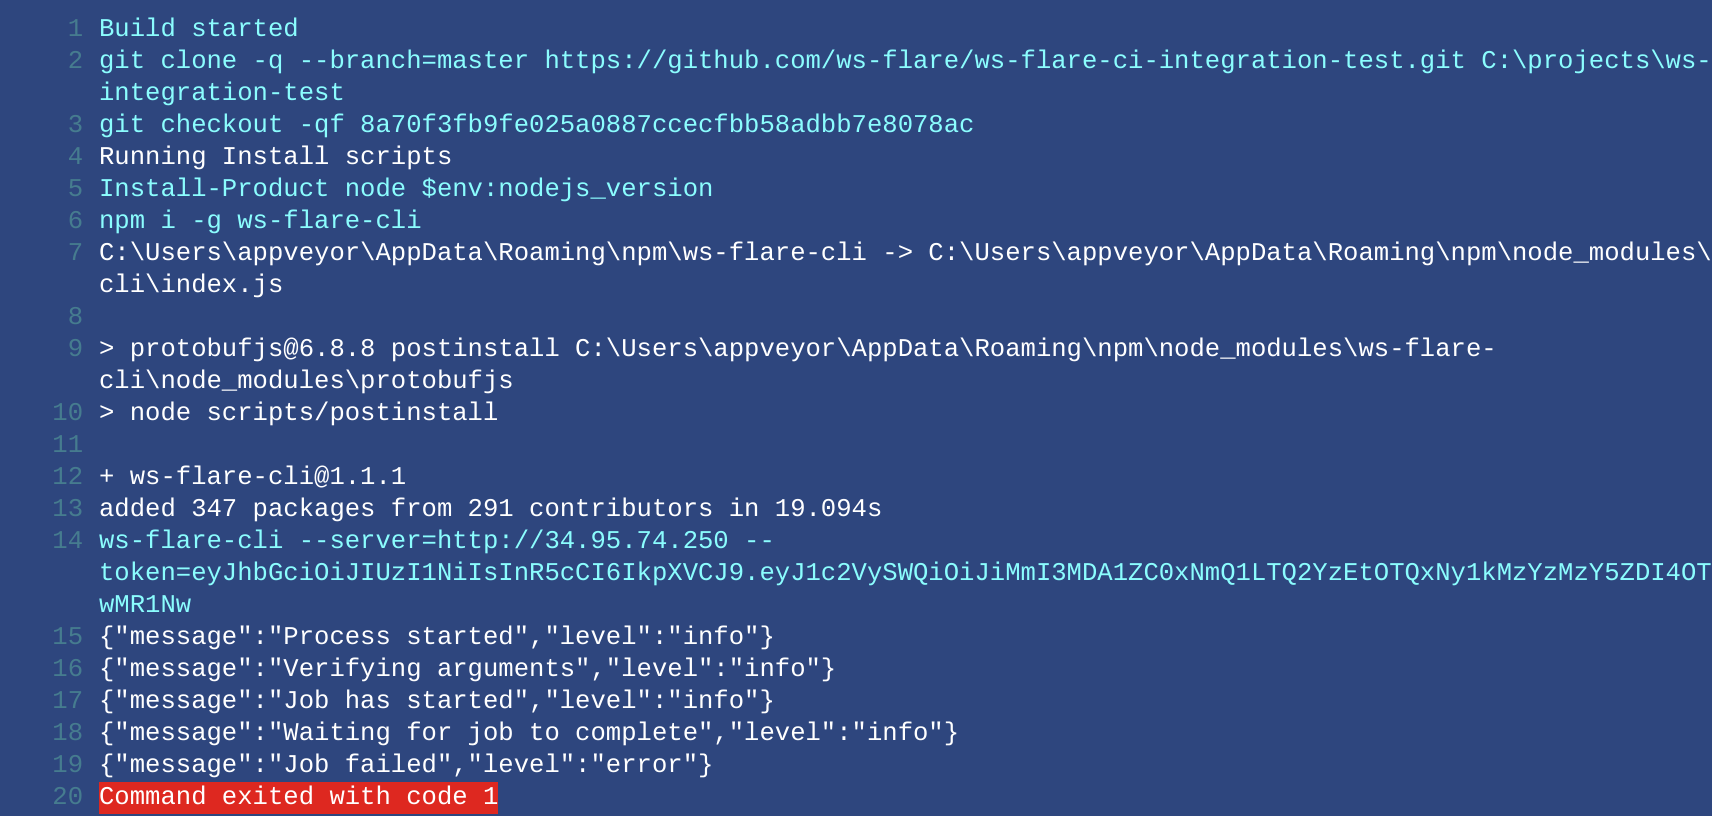
\includegraphics[width=1\textwidth]{figures/experiments/experiment-3/appveyor-output-failed.png}
    \caption{Failed Appveryor build when running ws-flare-cli command}
    \label{fig:experiment-3-appveyor-log-failed}
\end{figure}